\documentclass[doublespace,Afour,sageh]{sagej}
\usepackage{fontspec,xeCJK}
\setmainfont{lmroman10-regular.otf}[BoldFont=lmroman10-bold.otf,ItalicFont=lmroman10-italic.otf,BoldItalicFont=lmroman10-bolditalic.otf]
\setsansfont{lmsans10-regular.otf}[BoldFont=lmsans10-bold.otf,ItalicFont=lmsans10-oblique.otf,BoldItalicFont=lmsans10-boldoblique.otf]
\setmonofont{lmmono10-regular.otf}
\setCJKmainfont[Path=../fonts/,AutoFakeBold=2,AutoFakeSlant=.12]{NotoSerifCJKsc-Regular.otf}
\setCJKsansfont[Path=../fonts/,AutoFakeBold=2,AutoFakeSlant=.12]{NotoSansCJKsc-Regular.otf}
\setCJKmonofont[Path=../fonts/,AutoFakeBold=2]{NotoSansCJKsc-Regular.otf}
\usepackage{amsmath,amssymb,amsthm,mathtools,graphicx,booktabs,array,url,tabularx,multirow}
\usepackage{microtype,etoolbox}
\usepackage{xr-hyper}
\usepackage[colorlinks,bookmarksopen,bookmarksnumbered,citecolor=blue,urlcolor=blue,linkcolor=blue]{hyperref}
% In the bundled TeX Live driver, named remote destinations can retain a
% previous page-action counter. A named destination has no page argument.
\makeatletter
\patchcmd{\hyper@linkfile}{\Hy@MakeRemoteAction}
  {\ifx\\#3\\\else\let\Hy@href@page\@empty\fi\Hy@MakeRemoteAction}
  {}{\errmessage{Named remote destination patch failed}}
\makeatother
\setcounter{secnumdepth}{3}
\setcounter{dbltopnumber}{2}
\renewcommand{\dbltopfraction}{0.90}
\renewcommand{\textfraction}{0.08}
\renewcommand{\floatpagefraction}{0.8}
\emergencystretch=2em
\renewcommand{\bibfont}{\fontsize{9}{11pt}\selectfont}
\setlength{\tabcolsep}{4pt}
\newcolumntype{Y}{>{\raggedright\arraybackslash}X}
\def\journalname{V10 整合修订稿}
\def\volumenumber{1}
\def\issuenumber{ZH}
\newcommand{\versionlanguage}{中文译稿，与英文定稿对应}
\runninghead{Birkhoff 离散化与残差控制}
\newtheorem{theorem}{定理}
\newtheorem{proposition}[theorem]{命题}
\newtheorem{lemma}[theorem]{引理}
\newtheorem{corollary}[theorem]{推论}
\theoremstyle{definition}
\newtheorem{assumption}{假设}
\newtheorem{remark}{注}
\newcommand{\R}{\mathbb R}
\newcommand{\C}{\mathbb C}
\newcommand{\T}{\mathbb T}
\newcommand{\dd}{\,\mathrm d}
\newcommand{\norm}[1]{\left\lVert#1\right\rVert}
\newcommand{\abs}[1]{\left|#1\right|}
\newcommand{\diag}{\operatorname{diag}}
\newcommand{\Rea}{\operatorname{Re}}
\newcommand{\Ima}{\operatorname{Im}}
\newcommand{\eps}{\varepsilon}
\providecommand{\doi}[1]{\href{https://doi.org/#1}{doi: #1}.}
\makeatletter
\def\@maketitle{%
\if@Royal
\vspace*{-20pt}
\fi
\if@Crown
\vspace*{-20pt}
\fi
\vspace*{-34pt}%
\null%
\begin{center}
\if@PCfour
\begin{rm}
\else
\begin{sf}
\fi
\begin{minipage}[t]{\textwidth-57.625mm}
  \vskip 12.5pt%
    {\raggedright\titlesize\textbf{\@title} \par}%
    \vskip 1.5em%
    \vskip 12.5mm%
    \end{minipage}\hspace{15mm}\begin{minipage}[t]{42.625mm}
\hbox{}\scriptsize\journalname\\
\hbox{}方向一研究框架整合\\
\hbox{}2026 年 10 月 28 日\\
\hbox{}\versionlanguage\\[4pt]
\hbox{}{\fboxsep 2pt\fbox{研究修订稿}}
\end{minipage}
{\par\large%
\if@Royal
      \vspace*{6mm}
      \fi
      \if@Crown
      \vspace*{6mm}
      \fi%
      \lineskip .5em%
      {\raggedright\textbf{\@author}
      \par}}
     \vskip 40pt%
    {\noindent\usebox\absbox\par}
    {\vspace{20pt}%
      %
      {\noindent\normalsize\@keywords}\par}
      \if@PCfour
      \end{rm}
      \else
      \end{sf}
      \fi
      \end{center}
      \if@Royal
      \vspace*{-4.5mm}
      \fi
      \if@Crown
      \vspace*{-4.5mm}
      \fi
      \vspace{22pt}
        \par%
  }
 
\makeatother


\renewcommand{\proofname}{证明}
\renewcommand{\tablename}{表}
\renewcommand{\figurename}{图}
\renewcommand{\refname}{{\normalsize 参考文献}}
\makeatletter
\patchcmd{\abstract}{Abstract}{摘要}{}{\errmessage{Abstract translation patch failed}}
\patchcmd{\keywords}{Keywords}{关键词}{}{\errmessage{Keywords translation patch failed}}
\makeatother

\externaldocument{supplement_xr}[v10_Integrated_ZH_Supplement.pdf]
\hypersetup{pdftitle={磁性导管模型的Birkhoff离散化与复哈密顿残差控制},pdfauthor={匿名作者},pdfsubject={V10与方向一研究框架整合，2026年10月28日}}
\begin{document}
\title{磁性导管模型的 Birkhoff 离散化\\与复哈密顿残差控制}
\author{匿名作者}
\begin{abstract}
磁性导管模型需要将力学降阶、学习补偿和数值动力学一致地连接起来。本文通过三个相互衔接的子问题建立这一联系：Birkhoff 差分格式的矩阵实现、保守残差辨识与磁输入实现，以及受控离散格式的结构和收敛。带端部磁体的平面梁提供统一且参数来源可追溯的模型，并保留完整的耦合余弦势和端部惯量。相容的含时正则表示导出加权中点映射，端点投影和非交换矩阵消元则明确它与普通中点格式的关系。利用状态的积分观测，在不使用加速度标签的条件下联合辨识解析势能残差和比例阻尼。所得补偿在同一个隐式更新中求值，并通过磁力和磁力矩实现。本文建立含有显式累积求解残差项的有限时间收敛估计，并将其与相对于标称目标的误差区分开来。当非保守残差被消除时，由隐式方程精确定义的映射是精确辛映射。闭环哈密顿量的四次正规形和学习误差预算进一步给出离散 KAM 持久性的条件性论证。线性矩阵检验和非线性磁控制实验分别检验三个子问题。全模态实现、执行器标定和有限振幅 KAM 证书仍需满足文中明确列出的附加要求。
\end{abstract}
\keywords{Birkhoff 系统，磁性导管控制，残差学习，几何积分，数值收敛，离散 KAM}
\maketitle
\raggedbottom
\section{研究背景与问题}\label{sec:background}
磁驱动通过磁场及其空间梯度向柔性体施加远程力和力矩 \citep{abbott,kim}。有效的控制模型需要将这些输入贯穿力学降阶、辨识和数值实现，并在各环节保持同一个动力学对象。本文针对平面夹持--自由磁性导管模型研究这一完整联系。应用背景允许忽略重力；当前基准则限定为小斜率、无接触且不承受周围流体载荷。向更一般情形扩展时，仍需从一般杆力学出发 \citep{simo,antman}。

非线性目标保留完整的耦合余弦磁势。本文不通过消去其高阶项将系统变成独立的线性振子，因为这些项正是持久性分析中非线性频率变化的来源。控制器围绕该标称目标，补偿已辨识的保守残差和比例阻尼。因此，核心问题是：同一学习补偿能否与维度正确的差分格式、物理磁指令，以及对所得离散动力学的严格陈述相衔接。

\subsection{三个相互衔接的子问题}
\label{fw:three-questions}
\textbf{P1：推导并实现差分格式。} 从相容的 Birkhoff 表示出发，哪些端点变量允许定义生成函数，由此得到什么矩阵更新？力学质量矩阵、相流 Jacobian 与端点变换具有不同的维度。将外观类似标量的公式实现为多模态算法时，必须区分这些对象。对于比例阻尼，加权保结构映射又不同于直接作用在有阻尼向量场上的普通中点法。本文明确给出这些构造，并在进入非线性导管模型之前检验非交换矩阵运算。

\textbf{P2：辨识并物理实现残差补偿。} 能否利用状态观测确定保守残差和阻尼估计，同时保留标称的耦合磁势？辨识、控制器和仿真对象必须使用同一坐标，而学习控制器不能读取生成合成数据时所用的未知系数。第二项要求来自物理实现：两个广义模态指令必须先经过统一的力--力矩接口，再重构为局部磁场--梯度。较小的辨识残差本身既不验证激励充分性，也不验证硬件可行性。

\textbf{P3：建立受控格式的结构与收敛。} 将反馈放入同一个中点方程之后，该格式逼近哪个向量场，辨识误差下还保留什么结构，非线性求解又如何影响收敛？有限时间误差必须相对于同一实际闭环计算；实际闭环与标称目标的偏差属于另一项模型误差。自治保守分支可以具有精确辛性，而离散 KAM 还要求解析域、非共振、扭转和定量小量条件。这些推论不能仅凭相图或较小的能量漂移得出。

\subsection{贯穿全文的同一物理与统计模型}
基准由文献材料参考值、磁体制造商规格和明确声明的几何及阻尼选择共同建立。Sylgard 184 参考值对应其发表文献中的配比与固化条件 \citep{cho2021pdms}，不代表当前梁组件的实测值。在求解含磁偏置的特征值问题之前，端部磁芯的平动和转动惯量已纳入模型。这些输入决定三个子问题共同使用的模态尺度、物理解码器和磁输入映射。参数来源见第~\ref{sec:derivation} 节和补充材料~\ref{sec:supp-mechanics}。

力学推导链与学习假设类保持明确区分。哈密顿神经网络学习标量能量，并由其导数决定向量场 \citep{greydanus}；单独表示耗散与驱动，才能保留有意义的功率平衡 \citep{zhong,desai}。复坐标用于组织实位置和动量通道，复特征也可提供具有结构的表示 \citep{trabelsi}。实能量同时依赖复坐标及其共轭；KAM 所需的解析延拓则将底层复化坐标视为独立变量。这一记号或通用逼近定理均不能为任意拟合网络提供经过验证的导数误差界 \citep{hornik,zhang}。

实际实现的实验固定已知动能，通过状态的积分观测联合学习解析势能残差和一个标量阻尼系数。实验使用一个明确声明的磁势特征，从而分别检验辨识误差、数值误差和输入重构。更大的解析读出仍属于理论框架，但本文计算不声称完成不受此限制的隐藏层训练，也不声称给出新的复网络与实网络性能比较。即使在单特征检验中，完整的标称余弦势也始终保留。

\subsection{几何分析与控制目标}
在几何条件和局部可逆性条件成立时，生成函数可构造经典的辛方法 \citep{feng,fengqin,hairer}。本文采用比例阻尼下的构造性 Birkhoff 表示，推导其端点投影与时间中点更新，并在保守极限下恢复普通哈密顿中点映射。四阶中心生成函数保留其完整修正项。本文将这些经典构造应用于所声明的力学与反馈模型，不主张提出新的通用积分方法。

控制器估计阻尼和势能修正，同时保留 $h_0$ 作为标称目标。实际闭环的保守部分为 $h_c=h_0+\delta R$，其中 $\delta R$ 是残差辨识误差。剩余阻尼必须作为非保守项保留。因此，即使精确辛性和经典 KAM 不成立，时间离散格式仍可能收敛。第~\ref{sec:analysis} 节将这一区分表述为受控数值分析结论，并明确包含隐式求解残差的累积效应。

磁势的四次正规形给出可计算的扭转，作为条件性持久性论证的基础。从学习到 KAM 的结论需要超出较小经验损失的假设 \citep{chen2022}，因此本文保留确定性的系数误差及解析误差预算。连续 KAM 为保守目标提供背景 \citep{poschel}，主要的离散结论则使用 \citet{shang} 的生成映射框架。有限振幅的后验认证还需要具体嵌入、不变性缺陷和几何界 \citep{haro2019aposteriori}。本研究中的数值诊断尚未给出这样的新证书。

相关磁机器人研究将降阶模型、视觉反馈和仿真接入物理控制 \citep{francescon2025shape,tong2025navigation}。本文集中研究引入这些附加感知与硬件层之前所需的解析和计算联系。学习一个保守参考并对其进行跟踪也是合理目标，但它产生不同的误差系统。该相关路线保留在补充材料~\ref{sec:supp-tracking}；主文始终围绕残差补偿目标展开。

\subsection{贡献与全文安排}
第一项贡献是从 Birkhoff 一形式、端点投影到矩阵实现的完整推导，并明确物理、模态和相空间的各级维度。第二项贡献是在耦合标称模型上，为残差补偿建立共同的积分辨识与磁输入实现构造。第三项贡献是对受控离散格式进行分析，区分有限时间收敛、精确或加权几何结构，以及条件性的离散 KAM 持久性。数值研究围绕相应接口组织，以分别检验这些联系。

\begin{table*}[t]
\centering
\caption{六节正文中的三个子问题。各行共用同一力学基准和补偿目标。}
\label{tab:roadmap}
\begin{tabularx}{\textwidth}{p{0.15\textwidth}YY}
\toprule
子问题 & 文中的构造 & 验证与适用边界\\
\midrule
P1：离散格式 & 第~\ref{sec:derivation} 节：相容 Birkhoff 形式、端点投影、矩阵中点及加权映射 & 第~\ref{sec:analysis} 节：独立矩阵指数参考、非交换消元及结构诊断\\
P2：学习控制 & 第~\ref{sec:derivation} 节：联合积分辨识与残差补偿；第~\ref{sec:application} 节：物理磁端口 & 第~\ref{sec:analysis} 节：同一对象上的四组控制消融；证据来自无噪声受限特征实验\\
P3：受控分析 & 第~\ref{sec:analysis} 节：隐式格式内的反馈与含求解残差的收敛；第~\ref{sec:kam} 节：离散持久性条件 & 固定模型误差与步长加密诊断；完整解析 KAM 预算及器件标定仍是独立要求\\
\bottomrule
\end{tabularx}
\end{table*}

第~\ref{sec:derivation} 节给出共同力学模型，以及离散格式和学习构造。第~\ref{sec:analysis} 节建立受控格式的有限时间性质，并报告三部分验证序列。第~\ref{sec:kam} 节将保守分支接入离散 KAM。第~\ref{sec:application} 节通过磁端口实现同一指令，并说明尚需满足的全梁和净空要求。第~\ref{sec:conclusion} 节总结对 P1--P3 的回答。补充材料提供详细证明、数值协议及相关的跟踪扩展。

\section{力学降阶与 Birkhoff 生成函数构造}\label{sec:derivation}
\subsection{变分力学与保守项、受迫项的分离}
\label{mech:variational}
残差补偿构造在降维、辨识、离散和驱动中始终使用同一个力学对象。
首先给出一般变分模型，再将其具体化为动能已知的两模态磁驱动梁。
控制目标保留耦合磁势；学习项表示保守势能残差和有效阻尼率。
下文的参数选值用于确定这一对象及其物理输入尺度。

力学建模从中心线为 $r(s,t)$、截面标架为 $D(s,t)\in SO(3)$ 的杆出发，
其中 $s\in[0,L]$ 为参考弧长。满足本质边界条件及所施加杆约束的构形映射
$(r(s,q),D(s,q))$ 同时确定平动动能和转动动能 \citep{simo,antman}。
空间降维后，记
\begin{equation}
 T=\tfrac12\dot q^{\mathsf T}M(q)\dot q,\qquad V=V(q),
 \label{mech:general-energy}
\end{equation}
其中 $M(q)=M(q)^{\mathsf T}\succ0$。弹性和给定静磁场对 $V$ 作出贡献；
磁场的调制则向系统做功。对于永久磁偶极子，相互作用势 $-m\cdot B$ 给出
$\tau=m\times B$ 和 $F=\nabla(m\cdot B)$，其中空间求导时保持取向不变
\citep{abbott}。

令 $c_{\rm geo}(q,\dot q)$ 为 $M$ 的导数产生的惯性项，
$\mathcal D_N(q,\dot q)$ 为瑞利耗散势，$B_u(q)u$ 表示广义控制力。
变分方程及其勒让德变换为
\begin{align}
 M\ddot q+c_{\rm geo}+\nabla V
 &=Q_{\rm drv}-\partial_{\dot q}\mathcal D_N+B_u u,
 \label{mech:general-lagrange}\\
 p&=M(q)\dot q,\qquad
 H=\tfrac12p^{\mathsf T}M(q)^{-1}p+V,\nonumber\\
 \dot q&=H_p,\qquad v=H_p,\nonumber\\
 \dot p&=-H_q-\partial_v\mathcal D_N(q,v)+Q_{\rm drv}+B_u u.
 \label{mech:general-hamiltonian}
\end{align}
特别地，$(H_q)_i$ 包含 $p^{\mathsf T}(\partial_{q_i}M^{-1})p/2$。
几何惯性并非额外的耗散力。在相应模型明确后，流体作用、移动边界做功和接触损失
可保留在 $Q_{\rm drv}$ 中。补充材料~\ref{sm:general} 的推导保留了这些区别，
其中也包括运动流体可以向杆提供机械能这一事实。
下文的解析持续性结果仅限于光滑、无接触的邻域。

\subsection{以文献为依据的物理基准}
\label{mech:benchmark}
为获得可复现的实例，将上述表述具体化为平面内的均匀圆截面悬臂梁，
并在远端附加刚性磁芯。该模型根部固定，无横向重力、外部流动、接触或流体附加质量。
这是以远程操控（包括微重力场景）为动机的无重力力学基准，
并非针对特定患者的导管模型。Euler--Bernoulli 运动学忽略剪切变形和分布式转动惯量。
端部转角近似为 $\vartheta=w_s(L,t)$；保留其三角函数形式的磁势能，
并不消除这一小斜率近似。

以 $\zeta_j^{\mathrm{d}}$ 表示模态阻尼比。
表~\ref{mech:parameters} 区分了实测材料参考值、标称磁性规格和设计选值。
Sylgard 184 参考材料采用约 $10$ wt\% 的固化剂，
在 $80\,^{\circ}\mathrm C$ 下固化 $2$ h \citep{cho2021pdms}。
文献报告的 $E$ 和密度是该制备条件下的近似参考值，并非本文圆柱试件的实测值。
固化剂质量分数为 $10$ wt\% 时，基料与固化剂的质量比约为 $9{:}1$，而非 $10{:}1$。

\begin{table*}[t]
\centering\small
\caption{修订后力学基准的输入参数。标为设计选值或情景的数值均非实验估计。}
\label{mech:parameters}
\setlength{\tabcolsep}{5pt}
\begin{tabular}{p{0.27\textwidth}p{0.22\textwidth}p{0.44\textwidth}}
\toprule
物理量 & 数值 & 依据与解释\\
\midrule
梁长 $L$、半径 $r$ & $80$ mm、$0.6$ mm & 均匀实心梁的指定几何尺寸。\\
杨氏模量 $E$ & 约 $2.1$ MPa & Sylgard 184 材料参考值，制备条件见正文 \citep{cho2021pdms}。\\
质量密度 $\rho$ & 约 $1028\,\mathrm{kg\,m^{-3}}$ & 同一材料参考文献 \citep{cho2021pdms}；不声称已对同批试件进行标定。\\
裸磁芯边长 $a_m$ & $0.250$ mm & 指定的立方磁芯设计；不计涂层和胶黏剂。\\
剩余磁通密度 $B_r$ & 标称值 $1.425$ T & N50 牌号范围 $1.40$--$1.45$ T 的中点 \citep{smN50}。\\
磁芯密度 $\rho_m$ & 标称值 $7500\,\mathrm{kg\,m^{-3}}$ & 取制造商声明的规格下限；并非单个磁芯的密度实测值 \citep{smN50}。\\
轴向偏置场 $B_0$ & $30$ mT & 设计选值；已发表的 OctoMag 实验提供了 $40$ mT 矢量磁场能力的参照 \citep{lussi2021cvs}。\\
第一模态阻尼比 $\zeta_1^{\mathrm{d}}$ & $0.025$ & 有效阻尼情景，相对于包含端部惯量的偏置场下频率定义。\\
有效中心线净空 $c$ & $4$ mm & 设计比较值，已从通道半宽中扣除杆半径。\\
\bottomrule
\end{tabular}
\end{table*}

对于均匀磁化的硬磁芯，采用工程近似 $\mu\simeq B_ra_m^3/\mu_0$，
其中 $\mu_0\simeq4\pi10^{-7}\,\mathrm{H\,m^{-1}}$ \citep{kjMoment}。
标称磁偶极矩及惯性参数为
\begin{align}
 \mu&=1.77184214\times10^{-5}\,\mathrm{A\,m^2},\nonumber\\
 m_t=\rho_ma_m^3&=1.171875\times10^{-7}\,\mathrm{kg},\nonumber\\
 J_t=m_ta_m^2/6&=1.220703125\times10^{-15}\,\mathrm{kg\,m^2}.
 \label{mech:core-properties}
\end{align}
将磁芯质心理想化为位于梁端点。偏心安装会引入惯性耦合，并改变载荷力臂。
该磁偶极矩估计不表征实际装置的磁化历史、涂层或制造公差。
这些假设定义了一个自洽的数值对象，没有混用不同复合材料机器人的材料参数。

\subsection{边界惯量、有限元与储存能量}
\label{mech:finite-elements}
令 $A_c=\pi r^2$、$I=\pi r^4/4$，并采用有效阻尼模型 $C=\alpha M_f$。
对应连续梁的内部方程和固支边界条件为
\begin{align}
 \rho A_cw_{tt}+\alpha\rho A_cw_t+EIw_{ssss}&=0,\nonumber\\
 w(0,t)=w_s(0,t)&=0.
 \label{mech:beam}
\end{align}
以 $F$ 表示横向端力，$\tau_B=\mu B_y\cos\vartheta$ 表示主动端部磁力矩，
自然端部平衡条件为
\begin{align}
 -EIw_{sss}(L)&=F-m_t[w_{tt}(L)+\alpha w_t(L)],\nonumber\\
 EIw_{ss}(L)&=\tau_B-\mu B_0\sin\vartheta\nonumber\\
 &\quad-J_t(\ddot\vartheta+\alpha\dot\vartheta).
 \label{mech:endpoint-balance}
\end{align}
因此，端部转动仍是自由的。端部阻尼项属于所声明的 $C=\alpha M_f$ 近似，
并非对磁芯损耗的独立测量。

令 $q$ 汇集不受约束的 Hermite 位移和斜率坐标，
$e_w,e_\vartheta$ 分别选取其端部值。由弱形式得到
\begin{align}
 M_f&=M_{\rm beam}+m_te_we_w^{\mathsf T}
                         +J_te_\vartheta e_\vartheta^{\mathsf T},\nonumber\\
 M_f\ddot q+\alpha M_f\dot q+K_{\rm beam}q
 &=e_wF+e_\vartheta(\tau_B-\mu B_0\sin\vartheta),\nonumber\\
 \vartheta&=e_\vartheta^{\mathsf T}q.
 \label{mech:fe-plant}
\end{align}
取 $p=M_f\dot q$ 和 $E_0=\mu B_0$，标称物理哈密顿量为
\begin{align}
 H_0(q,p)&=\tfrac12p^{\mathsf T}M_f^{-1}p
             +\tfrac12q^{\mathsf T}K_{\rm beam}q\nonumber\\
 &\quad+E_0[1-\cos\vartheta].
 \label{mech:fe-energy}
\end{align}
这里 $E_0=5.31552642\times10^{-7}\,\mathrm J$。
偏置场储存能量，而 $F$ 和 $B_y$ 通过不同的物理端口做功。其功率平衡为
\begin{equation}
 \dot H_0=-\alpha\dot q^{\mathsf T}M_f\dot q
              +F\dot w(L)+\tau_B\dot\vartheta.
 \label{mech:physical-power}
\end{equation}

计算采用 $32$ 个一致质量三次 Hermite 单元和 $64$ 个自由节点坐标。
补充材料~\ref{sm:fe-check} 给出的独立端部特征方程以及 $16/32/64$ 单元比较，
验证了前两阶频率的相对误差分别为 $9.02\times10^{-9}$ 和 $3.29\times10^{-7}$，
对应 $32$ 个单元的离散。
该检验针对线性离散精度；后续限制到两模态仍是另一项模型降阶。

\subsection{质量归一化与正则缩放}
\label{mech:canonical}
将静磁场项线性化，得到
\begin{align}
 K_b&=K_{\rm beam}+E_0e_\vartheta e_\vartheta^{\mathsf T},\nonumber\\
 K_b\Phi_n&=M_f\Phi_n\Omega_n^2,\qquad
 \Phi_n^{\mathsf T}M_f\Phi_n=I_n,
 \label{mech:modal-bias}
\end{align}
其中 $\Omega_n=\diag(\omega_1,\ldots,\omega_n)$。
令 $q=\Phi_na$，则模态动量为 $\pi=\dot a$。
只有经过该归一化，模态质量矩阵才是 $I_n$。
设 $\omega_0=\omega_1$、$\tau=\omega_0t$、
$\nu_j=\omega_j/\omega_0$ 和 $\mathsf N=\diag(\nu_j)$。
平衡正则缩放为
\begin{align}
 a_j&=S_jX_j,\qquad S_j=\sqrt{\frac{E_0}{\omega_0\omega_j}},\nonumber\\
 \pi_j&=\sqrt{\frac{E_0\omega_j}{\omega_0}}Y_j,
 \qquad D_s=\diag(S_j).
 \label{mech:scaling}
\end{align}
位置与动量尺度的乘积为 $E_0/\omega_0$。
结合能量 $H_0/E_0$ 和时间 $\tau$，即可得到正则无量纲方程，
而不是将 $M_f$ 替换为单位质量。对于 Hermite 插值行向量 $N_w(s)$，定义
\begin{equation}
 \ell(s)^{\mathsf T}=N_w(s)\Phi_nD_s,\qquad
 d=D_s\Phi_n^{\mathsf T}e_\vartheta.
 \label{mech:shape-maps}
\end{equation}
于是 $w(s)=\ell(s)^{\mathsf T}X$、$\vartheta=d^{\mathsf T}X$，且
\begin{align}
 h_0(X,Y)&=h_2(X,Y)+g(d^{\mathsf T}X),\nonumber\\
 h_2&=\tfrac12(X^{\mathsf T}\mathsf NX+Y^{\mathsf T}\mathsf NY),\nonumber\\
 g(s)&=1-\cos s-\tfrac12s^2.
 \label{mech:nominal-energy}
\end{align}
减去二次项是为避免重复计入偏置刚度。对于两模态实例，
\begin{align}
 \omega_0&=7.84000916\,\mathrm{rad\,s^{-1}},\nonumber\\
 \nu&=(1,6.04585730)^{\mathsf T},\nonumber\\
 d&=(0.30722439,0.45042632)^{\mathsf T},\nonumber\\
 \ell(L)&=(0.0189673443,0.00775347614)^{\mathsf T}\,\mathrm m.
 \label{mech:reduced-values}
\end{align}
导出的系数保留了比此处显示值更多的位数。
额外位数用于标识该数值基准，并不意味着具有相应的测量精度。
在 $(X,Y,\tau)$ 中，有效质量矩阵为 $\mathsf N^{-1}$。
表~\ref{mech:dimension-table} 集中列出残差控制器及其离散所用的坐标层级。
$32$ 单元模型具有 $64$ 个构形坐标和 $128$ 维相空间。
将其质量归一化模态族限制为 $n=2$ 时，质量矩阵为 $I_2$；
随后作平衡缩放，得到 $M_{\rm eff}=\mathsf N^{-1}$。
各质量矩阵均对应其所声明的坐标。
对于一般的 $n$ 模态模型，相流 Jacobian $D\Phi$ 的尺寸为 $2n\times2n$，
联合端点变换的尺寸为 $4n\times4n$；在受控两模态系统中，
这两个尺寸分别为 $4\times4$ 和 $8\times8$。
补充材料~\ref{ss:projection} 给出生成函数使用的端点投影。

\begin{table*}[t]
\centering\small
\caption{同一力学基准的坐标层级。质量归一化和平衡缩放是两个独立的变换步骤。}
\label{mech:dimension-table}
\setlength{\tabcolsep}{5pt}
\begin{tabular}{p{.22\textwidth}p{.24\textwidth}p{.22\textwidth}p{.23\textwidth}}
\toprule
层级 & 坐标与时间 & 动能质量矩阵 & 相空间状态与切映射尺寸\\
\midrule
完整 $32$ 单元梁 & $q,p\in\mathbb R^{64}$，物理时间 $t$ & $M_f\in\mathbb R^{64\times64}$，包含 $m_t,J_t$ & $128$；$D\Phi\in\mathbb R^{128\times128}$\\
质量归一化的 $n$ 个模态 & $a,\pi\in\mathbb R^n$，物理时间 $t$ & $I_n$；$I_2$ 对应 $n=2$ & $2n$；$D\Phi\in\mathbb R^{2n\times2n}$\\
平衡缩放的两模态控制器 & $X,Y\in\mathbb R^2$，$\tau=\omega_0t$ & $M_{\rm eff}=\mathsf N^{-1}$ & $4$；$D\Psi_\Delta\in\mathbb R^{4\times4}$\\
\bottomrule
\end{tabular}
\end{table*}

阻尼情景取 $\alpha=2\zeta_1^{\mathrm{d}}\omega_0=0.3920004581\,\mathrm{s^{-1}}$ 和
$\gamma=\alpha/\omega_0=0.05$；这并不使每个模态具有相同的阻尼比。
其他阻尼比作为明确声明的情景进行研究，不用不同条件下测得的材料损耗因子替代模态阻尼。

\subsection{复坐标、耗散与物理输入}
\label{mech:complex}
令 $x=(X,Y)$ 且 $J=\left(\begin{smallmatrix}0&I\\-I&0\end{smallmatrix}\right)$。
可逆的复坐标图为
\begin{equation}
 \zeta=(X+\mathrm iY)/\sqrt2,\qquad
 \chi=(X-\mathrm iY)/\sqrt2.
 \label{mech:complex-chart}
\end{equation}
在实相空间上，$\chi=\bar\zeta$。将 $\zeta,\chi$ 视为相互独立的复变量，
得到整函数延拓
\begin{equation}
 h_0^{\mathbb C}(\zeta,\chi)
 =\sum_j\nu_j\zeta_j\chi_j
       +g\!\left(d^{\mathsf T}(\zeta+\chi)/\sqrt2\right).
 \label{mech:complex-energy}
\end{equation}
采用约定 $\{\zeta_j,\bar\zeta_k\}=-\mathrm i\delta_{jk}$，则
\begin{align}
 \partial_{\bar\zeta}&=(\partial_X+\mathrm i\partial_Y)/\sqrt2,\nonumber\\
 \zeta'&=-\mathrm i\partial_\chi h^{\mathbb C},\qquad
 \chi'=\mathrm i\partial_\zeta h^{\mathbb C}.
 \label{mech:wirtinger}
\end{align}
关于两个独立复变量的解析延拓，才是解析 KAM 理论使用的对象；
实值能量不必仅关于 $\zeta$ 一个变量全纯。

复哈密顿神经表示提供实值能量读出 $h_\eta$ 和无量纲耗散读出
$\mathcal D_\eta(X,v)$，后者由物理瑞利耗散势除以 $E_0\omega_0$ 得到。
其动力学显式定义为
\begin{align}
 X'&=v=\partial_Yh_\eta,\nonumber\\
 Y'&=-\partial_Xh_\eta-\partial_v\mathcal D_\eta(X,v)+U.
 \label{mech:decoder}
\end{align}
先对速度求导，再代入 $v=\partial_Yh_\eta$。
例如，取 $\mathcal D_\eta=\widehat\gamma v^{\mathsf T}\mathsf N^{-1}v/2$、
$\widehat\gamma\ge0$，得到
\begin{equation}
 h_\eta'=-v^{\mathsf T}\partial_v\mathcal D_\eta+v^{\mathsf T}U,
 \label{mech:power}
\end{equation}
当参数随时间变化时，还需加上 $\partial_\tau h_\eta$。
因此，$h_\eta+\mathrm i\mathcal D_\eta$ 是一对经解码的读出，
不同于解析延拓 $h_\eta^{\mathbb C}$。
复记号下的非保守项为 $\mathrm i[-\partial_v\mathcal D_\eta+U]/\sqrt2$。

对于动能形式固定的两模态模型，令
$b_j=e_w^{\mathsf T}\phi_j$、$t_j=e_\vartheta^{\mathsf T}\phi_j$。
物理输入换算为
\begin{align}
 A_{\rm mag}&=\begin{pmatrix}b_1&t_1\\b_2&t_2\end{pmatrix},
 &\Lambda&=\omega_0^2D_s\mathsf N=E_0D_s^{-1},\nonumber\\
 \Lambda U&=A_{\rm mag}\binom{F}{\tau_B}.
 \label{mech:modal-ports}
\end{align}
仅有均匀横向磁场时，$U=(B_y/B_0)d\cos\vartheta$，只提供一个输入方向。
要实现一般的二维向量 $U$，必须具备独立调节磁场及其梯度的能力。
第~\ref{sec:application} 节将这一接口用于学习得到的残差补偿律，
并考察同一控制律在包含更多模态的受控对象上的作用。
针对一般目标哈密顿量（包括学习得到的动量项）的更强实现另见
补充材料~\ref{sm:exact-lift}；跟踪扩展在补充材料第~\ref{sec:supp-tracking} 节使用同一接口。

\subsection{力学模型的相容 Birkhoff 表示}
\label{struct:birkhoff-section}

第一个子问题是从定义导管的同一组力学方程出发，得到可计算的差分格式。式 \eqref{mech:general-hamiltonian} 中的一般模型将保守能量、耗散和外加力分开。对于 $z=(q,p)\in\R^{2n}$，Birkhoff 表示采用一形式 $\mathcal R(z,t)^{\mathsf T}\dd z$ 和标量 $\mathcal B$：
\begin{equation}\label{struct:birkhoff}
\begin{aligned}
 \mathcal K_{ij}&=\partial_{z_i}\mathcal R_j-
                  \partial_{z_j}\mathcal R_i,\\
 \mathcal K\dot z&=\nabla_z\mathcal B+\partial_t\mathcal R=:b.
\end{aligned}
\end{equation}
其中，$\mathcal K$ 必须非奇异且反对称，其矩阵元与 $b$ 还须满足
\begin{equation}\label{struct:compatibility}
\begin{aligned}
 \partial_k\mathcal K_{ij}+\partial_i\mathcal K_{jk}
                +\partial_j\mathcal K_{ki}&=0,\\
 \partial_t\mathcal K_{ij}&=\partial_i b_j-\partial_j b_i.
\end{aligned}
\end{equation}
这些条件将一形式、标量和向量场联系起来；不能通过彼此独立地指定它们来表示任意耗散力 \citep{su2007}。Birkhoff 矩阵的尺寸为 $2n\times2n$，质量矩阵的尺寸则为 $n\times n$。表~\ref{mech:dimension-table} 列出了有限元、模态和平衡坐标下的维度。补充材料~\ref{ss:birkhoff} 给出相容性论证，并区分形式上的局部存在性构造与本文采用的显式表示。

对于比例动量阻尼 $\dot p=-H_q-\alpha(t)p$，令 $a(t)=\exp\!\int_{t_0}^{t}\alpha(s)\dd s$。一种可构造的相容选择为
\begin{equation}\label{struct:weighted-hamiltonian}
\begin{aligned}
 \mathcal R&=(a p,0),\qquad \mathcal B=aH,
       \qquad\mathcal K=-aJ,\\
 \Pi&=a p,\qquad
 \widetilde H(q,\Pi,t)=a(t)H(q,\Pi/a(t),t).
\end{aligned}
\end{equation}
它恢复原方程，并使 $Z=(q,\Pi)$ 成为正则变量。只要保留 $M=M(q)$ 情形下 $H_q$ 中的全部质量导数，这一构造就允许质量随位置变化。$\widetilde H$ 的时间依赖性及向物理动量的变换承载了阻尼；仅凭这一表示，还不能得到经典 KAM 理论所需的自治保守系统。

\subsection{端点投影与生成函数构造}
\label{struct:endpoint-section}

端点构造及其时间展开分别承担原框架中定理 A 和定理 B 的作用 \citep{feng,fengqin}。这里给出当前实现所需的局部论证，不要求所生成的梯度本身可逆。记 $\lambda_Z=\Pi^{\mathsf T}\dd q$。若端点变换 $\alpha:(Z_+,Z_-)\mapsto(\widehat w,w)$ 局部可逆，并满足
\[
 \dd(\widehat w^{\mathsf T}\dd w)
      =\dd\lambda_{Z_+}-\dd\lambda_{Z_-}.
\]
则称其相容。

\begin{proposition}[端点投影：定理 A 的作用]
\label{struct:endpoint-proposition}
设 $Z_+=\Phi_Z(Z_-)$ 是固定时间端点之间的辛映射图像。假设相容变换 $\alpha$ 的下方导数分块为 $C_\alpha,D_\alpha$，并满足
\[
 \det\bigl(C_\alpha D\Phi_Z+D_\alpha\bigr)\ne0.
\]
则在充分小的单连通邻域内，该图像可以写成 $\widehat w=\nabla_w\varphi(w)$。这里不要求 $\partial_w\widehat w$ 可逆。
\end{proposition}

\begin{proof}
上述投影条件使 $w$ 成为图像上的局部坐标。辛性与相容性使 $\widehat w^{\mathsf T}\dd w$ 在该图像上闭合，再由局部 Poincar\'e 引理得到标量 $\varphi$。这些步骤使用的是到 $w$ 的投影，不是其梯度的逆。
\end{proof}

在中央端点约定下，令 $T_0=\diag(I_n,-I_n)$、$\mathsf E=\left(\begin{smallmatrix}0&I_n\\I_n&0\end{smallmatrix}\right)$，并选择
\begin{equation}\label{struct:endpoint-variables}
\begin{aligned}
 \widehat w&=(\widehat Q,\widehat P)=\mathsf E(Z_+-Z_-),\\
 w&=T_0\bar Z=(Q,P)=(\bar q,-\bar\Pi).
\end{aligned}
\end{equation}
其完整导数的尺寸为 $4n\times4n$，其中 $C_\alpha=D_\alpha=T_0/2$，故
\begin{equation}\label{struct:endpoint-projection}
 D_{Z_-}w=\tfrac12T_0(D\Phi_Z+I_{2n}).
\end{equation}
零步长时该矩阵为 $T_0$，因此在固定紧邻域内，步长充分小时仍可逆。相较之下，$\widehat w=f(w)$ 在零步长时恒为零，且 $f_w=0$。补充材料~\ref{ss:projection} 验证相容性、端点变量的联合逆变换以及它们与 Newton 矩阵的联系。

定理 B 的作用是将端点生成函数的时间展开转化为差分格式。对于含时哈密顿量，采用完整的时间中点 $t_m=t_k+\Delta_t/2$，并取
\begin{equation}\label{struct:lifted-generator}
\begin{aligned}
 \varphi_{\Delta_t}(Q,P)&=-\Delta_t\widetilde H(Q,-P,t_m),\\
 \widehat Q&=-\Delta_t\widetilde H_q(Q,-P,t_m),\\
 \widehat P&=\Delta_t\widetilde H_\Pi(Q,-P,t_m).
\end{aligned}
\end{equation}
代入式 \eqref{struct:endpoint-variables} 即得到正则时间中点方程。对于常数 $\alpha$ 和常质量，令 $r=\exp(\alpha\Delta_t/2)$，消去含绝对时间的指数项，得到
\begin{equation}\label{struct:weighted-midpoint}
\begin{aligned}
 q_+-q_-&=\tfrac{\Delta_t}{2}M^{-1}(r p_++r^{-1}p_-),\\
 r p_+-r^{-1}p_-&=-\Delta_t\nabla V\bigl((q_++q_-)/2\bigr).
\end{aligned}
\end{equation}
精确隐式映射满足
\begin{equation}\label{struct:weighted-structure}
\begin{aligned}
 (D\Phi)^{\mathsf T}J D\Phi&=e^{-\alpha\Delta_t}J,\\
 (D\Phi)^{\mathsf T}\mathcal K(t_+)D\Phi&=\mathcal K(t_-).
\end{aligned}
\end{equation}
这是 $Z$ 中的正则辛性经 $T_t(q,p)=(q,e^{\alpha t}p)$ 拉回所得的关系。完整的时间中点求值给出二阶一致性；若将显式时间依赖冻结在 $t_k$，可能只剩一阶。变质量时，同一构造仍适用于完整的 $\widetilde H$，但不能原样复用式 \eqref{struct:weighted-midpoint} 中的两条常质量更新式。

\subsection{普通中点格式与非交换矩阵}
\label{struct:matrix-section}

利用端点平均，也可对一般物理向量场作普通中点离散：
\begin{equation}\label{struct:mechanical-midpoint}
\begin{aligned}
 q_+-q_-&=\Delta_t M(\bar q)^{-1}\bar p,\\
 p_+-p_-&=\Delta_t[-H_q(\bar q,\bar p)-C_m\bar v]\\
           &\quad+\Delta_t(F_m+U_m),\\
 \bar v&=M(\bar q)^{-1}\bar p.
\end{aligned}
\end{equation}
所有状态相关量均在同一中点求值，所有显式时间参数均取 $t_m$。这恢复了原矩阵更新的完整向量形式。存在一般阻尼时，它与式 \eqref{struct:weighted-midpoint} 不同；二阶精度并不意味着具有式 \eqref{struct:weighted-structure} 中的指数结构因子。

对于常矩阵 $M,C,K$，设 $M\succ0$、$K=K^{\mathsf T}$、$V(q)=q^{\mathsf T}Kq/2$，消去位置中点得到
\begin{equation}\label{struct:matrix-elimination}
\begin{aligned}
 E_{\Delta_t}&=\tfrac{\Delta_t^2}{4}KM^{-1}
                         +\tfrac{\Delta_t}{2}CM^{-1},\\
 (I_n+E_{\Delta_t})p_+
    &=(I_n-E_{\Delta_t})p_--\Delta_tKq_-\\
    &\quad+\Delta_t(F_m+U_m),\\
 q_+&=q_-+\tfrac{\Delta_t}{2}M^{-1}(p_++p_-).
\end{aligned}
\end{equation}
矩阵次序 $KM^{-1}$ 来自将 $\bar q=q_-+\Delta_tM^{-1}(p_++p_-)/4$ 代入动量方程，推导不假设矩阵可交换。实现时求解系数矩阵为 $I_n+E_{\Delta_t}$ 的线性方程组，步长充分小时可保证其可逆。若反馈依赖未知中点，问题仍然是隐式的。对于 $M=M(q)$，还必须保留惯性向量 $-(\bar p^{\mathsf T}\partial_{q_i}M^{-1}\bar p)/2$，此时适宜直接求解 $2n$ 维残差方程。补充材料~\ref{ss:matrix} 给出完整消元过程。

在导管的平衡坐标中，应作如下代换：
\begin{equation}\label{struct:effective-matrices}
\begin{aligned}
 q&=X,\qquad p=Y,\\
 M_{\rm eff}&=\mathsf N^{-1},\qquad
 C_{\rm eff}=\gamma\mathsf N^{-1}.
\end{aligned}
\end{equation}
于是 $M_{\rm eff}^{-1}Y=\mathsf N Y$、$C_{\rm eff}M_{\rm eff}^{-1}Y=\gamma Y$。磁力仍为非线性，因此实际检验求解完整残差方程，不以常矩阵 $K$ 替代余弦势。第~\ref{sec:analysis} 节先以矩阵指数为参考检验非交换线性代数，再将同一离散方法用于该耦合磁模型。

\subsection{中央生成函数与自治高阶扩展}
\label{struct:schemes}

对于自治哈密顿量 $h$，采用状态 $x=(X,Y)$ 和无量纲时间 $\tau$，令 $f=J\nabla h$，并以 $\Delta$ 表示步长。中央约定为
\begin{equation}\label{struct:central-map}
 x_+-x_-=J\nabla S_\Delta(m),\qquad m=(x_++x_-)/2.
\end{equation}
通过 $\varphi_\Delta(Q,P)=-S_\Delta(Q,-P)$，它与前述端点记号等价。选择 $S_\Delta=\Delta h$ 得到
\begin{equation}\label{struct:midpoint}
 x_+-x_-=\Delta J\nabla h(m).
\end{equation}
当隐式方程存在唯一局部分支时，其 Jacobian 为
\begin{equation}\label{struct:cayley}
 D\Psi_\Delta=(I-C_\Delta)^{-1}(I+C_\Delta),\qquad
 C_\Delta=\tfrac12J S_\Delta''(m).
\end{equation}
$S_\Delta''$ 的对称性给出辛性。取 $\lambda=Y^{\mathsf T}\dd X$，对应的单值原函数为
\begin{equation}\label{struct:exact-symplectic}
 \Psi_\Delta^*\lambda-\lambda
 =\dd\bigl[\bar Y^{\mathsf T}(X_+-X_-)-S_\Delta(m)\bigr].
\end{equation}
因此该映射是\emph{精确辛}的。这一更强性质提供离散 KAM 所需的周期生成函数；它针对精确隐式映射，而不是采用有限容差的求解器输出。

保留中央时间展开中的下一个非零项，得到四阶扩展 \citep{feng}：
\begin{equation}\label{struct:central4}
 S_\Delta^{[4]}(x)=\Delta h(x)
       +\frac{\Delta^3}{24}f(x)^{\mathsf T}h''(x)f(x).
\end{equation}
补充材料~\ref{ss:central4} 推导其局部 $O(\Delta^5)$ 缺陷及谐振子相位公式。仅采用中点生成函数仍为二阶。若要得到四阶受控方法，式 \eqref{struct:central4} 必须使用实际自治闭环哈密顿量的全部导数。在一次 Central4 步之后另加控制增量，并不能建立该阶数或结构结论。

新参数下的主要闭环计算对实际向量场采用普通隐式中点法，
\begin{equation}\label{struct:general-midpoint}
 x_+-x_-=\Delta f_{\rm cl}(m,\tau_m).
\end{equation}
阻尼和反馈均在这一相同的未知中点求值。若同时积分参考轨迹，则将其纳入增广状态。式 \eqref{struct:midpoint} 是保守情形的特例；第~\ref{sec:analysis} 节将明确受控向量场何时具有该形式，并量化非精确隐式求解的影响。独立的线性检验和新参数非线性检验还针对保守目标 $h_0$ 验证 Central4，采用补充材料~\ref{ss:central4-magnetic-section} 中的显式导数。这些四阶检验并不赋予一般阻尼反馈闭环四阶精度或精确辛性。

\subsection{CHNN 模型类与四个哈密顿量}
\label{struct:objects-section}

式~\eqref{mech:complex-chart} 中的复变量用于组织哈密顿解码器；可训练对象仍是定义在真实物理状态空间上的实值能量。一般 CHNN 可通过复值隐藏层和实值读出来表示该能量，并使用独立的非负耗散分支。对应的力方程和功率方程为式~\eqref{mech:decoder}--\eqref{mech:power}。能量读出与耗散读出的作用不同：将二者的数值组合成一个复输出，并不会使耗散动力学成为哈密顿动力学。第~\ref{sec:kam} 节的 KAM 分析还要求能量在指定复邻域上具有解析性。

为明确辨识、力实现和误差估计，当前实现固定已知动能，并学习势能残差。令 $\mathsf N=\diag(\nu_1,\nu_2)$、$\vartheta=d^{\mathsf T}X$，定义
\begin{equation}\label{struct:objects}
\begin{aligned}
 g(s)&=1-\cos s-s^2/2,\\
 V_0(X)&=\tfrac12X^{\mathsf T}\mathsf N X+g(d^{\mathsf T}X),\\
 h_0(X,Y)&=\tfrac12Y^{\mathsf T}\mathsf N Y+V_0(X),\\
 h_*&=h_0+R_*,\qquad \widehat h=h_0+\widehat R,\\
 \delta R&=R_*-\widehat R,\qquad h_c=h_0+\delta R.
\end{aligned}
\end{equation}
四个能量分别对应标称模型、所声明模型类内的真实保守模型、学习模型，以及补偿闭环的保守部分。它们具有相同的二次动能，但势能不同。实际含阻尼和驱动的受控对象为
\begin{equation}\label{struct:plant}
 X'=\mathsf N Y,\qquad
 Y'=-\nabla(V_0+R_*)(X)-\gamma Y+U.
\end{equation}
未知质量、接触力或输入增益不由 $R_*(X)$ 表示；若包含这些效应，需要相应的模型和观测缺陷描述。

有限解析读出使一般 CHNN 架构可以直接核查：采用冻结的实解析特征，写成 $\widehat R(X)=\sum_{j=1}^{m}\widehat\beta_jF_j(X)$。最小实验取 $m=1$、$F_1=g(d^{\mathsf T}X)$，并设置人工真值系数 $\beta_*=0.2$。该系数是实验扰动，并非实测材料属性。架构中仍可保留这些特征的复值实现，但本次实验检验的是这一受限读出，并未训练不受限制的隐藏层。补充材料~\ref{ss:full-features} 给出完整的 $35$ 系数四次读出，并说明学习含动量项时增加的控制要求。

\subsection{能量与阻尼的联合积分辨识}
\label{struct:identification-section}

状态观测按互不重叠的整条轨迹划分为训练集和验证集。对每个观测窗口 $[a_\ell,b_\ell]$，令 $c_\ell=(c_{\ell X},c_{\ell Y})$ 为与端点匹配的重构曲线，$U_\ell^{\rm data}$ 为已知输入。记 $\mathcal V_F=[\nabla F_1,\ldots,\nabla F_m]$。对动量方程积分，得到
\begin{equation}\label{struct:integral-design}
\begin{aligned}
 y_\ell={}&c_{\ell Y}(b_\ell)-c_{\ell Y}(a_\ell)\\
   &+\int_{a_\ell}^{b_\ell}
      [\nabla V_0(c_{\ell X})-U_\ell^{\rm data}]\dd\tau,\\
 D_\ell={}&-\int_{a_\ell}^{b_\ell}
          [\mathcal V_F(c_{\ell X}),c_{\ell Y}]\dd\tau,\\
 \widehat\theta={}&(\widehat\beta_1,\ldots,\widehat\beta_m,
                      \widehat\gamma)^{\mathsf T}.
\end{aligned}
\end{equation}
堆叠后的设计矩阵有 $nL_I$ 行、$m+1$ 列；此处 $n=2$，$L_I$ 表示窗口数。使用 QR 或 SVD 求解来拟合 $D\theta\simeq y$，并通过奇异值诊断激励程度。施加 $\widehat\gamma\ge0$ 可得到满足被动性的物理阻尼估计。复算程序采用无约束线性求解，因此在零阻尼情景中出现的舍入量级负值作为数值拟合结果报告，不解释为物理负阻尼。

上述辨识不需要加速度标签。不过，端点噪声、插值、求积和未建模动力学仍会影响积分方程。它们进入需要独立界定的观测缺陷，不能由较小训练损失反推。第~\ref{sec:kam} 节将该缺陷及 Gram 下界转化为系数、力和解析能量的误差界。补偿控制器与补充材料~\ref{sec:supp-tracking} 中的跟踪扩展使用同一组冻结辨识结果和物理输入映射 \eqref{mech:modal-ports}。

\subsection{面向标称动力学的残差补偿}
\label{struct:route-a-section}

主要控制器在复现实验中记为路线 A。它抵消估计阻尼和势能残差，同时保留完整耦合的标称磁能量：
\begin{equation}\label{struct:route-a-control}
 U_A=\widehat\gamma Y+\nabla\widehat R(X).
\end{equation}
将其代入式 \eqref{struct:plant}，并令 $\delta\gamma=\gamma-\widehat\gamma$，得到
\begin{equation}\label{struct:route-a-closed}
 x'=J\nabla h_c(x)+\binom{0}{-\delta\gamma Y}.
\end{equation}
因此，非零保守学习误差将闭环哈密顿量变为 $h_c$，但不破坏 Hamiltonian 结构。非零阻尼误差则留下非保守项，其功率为 $h_c'=-\delta\gamma Y^{\mathsf T}\mathsf N Y$。由此，经典流或映射 KAM 只有在阻尼被精确抵消且指令广义力被精确实现时，才涉及这一物理闭环；另一种允许情形是将所有剩余力独立证明为自治势能梯度，并纳入 $h_c$。一般力误差即使很小，也不足以满足这一结构前提。

在精确补偿极限下，闭环为 $h_0$。路线 A 实验中的标称参考，是 $h_0$ 从同一初始状态出发的流。真值参数对照使用 $U=\gamma Y+\nabla R_*$，仅用于分离积分误差与辨识误差；学习控制器只使用拟合量。


下一节将这一反馈代入同一隐式方程，并证明相应结构和有限时间收敛性。跟踪学习得到的保守参考属于另一控制目标，保留在补充材料~\ref{sec:supp-tracking} 中。

\section{受控离散格式：收敛与数值验证}\label{sec:analysis}
\subsection{将反馈置于同一隐式方程中}
\label{ctrl:placement}

第二个子问题给出已辨识残差及其补偿。第三个子问题考察施加该反馈后形成何种差分格式、保留何种结构，以及数值轨迹如何逼近实际闭环动力学。这些问题针对第~\ref{sec:derivation} 节中的同一受控对象和同一未知中点。将式 \eqref{struct:route-a-control} 代入受控对象，得到受控更新式
\begin{equation}\label{ctrl:midpoint}
\begin{aligned}
 X_+-X_-&=\Delta\mathsf N\bar Y,\\
 Y_+-Y_-&=-\Delta\nabla(V_0+R_*)(\bar X)
               -\Delta\gamma\bar Y\\
        &\quad+\Delta U_A(\bar X,\bar Y)\\
        &=-\Delta\nabla(V_0+\delta R)(\bar X)
               -\Delta\delta\gamma\bar Y.
\end{aligned}
\end{equation}
因此，其连续时间目标为
$f_c(x)=J\nabla h_c(x)+(0,-\delta\gamma Y)^{\mathsf T}$，其中包含固定的辨识误差。连续广义力 $U_A\in\R^2$ 与其离散相空间贡献应加以区分：
\begin{equation}\label{ctrl:control-increment}
 \mathcal U_k=\Delta\binom{0}{U_A(\bar X,\bar Y)}\in\R^4.
\end{equation}
这种控制放置方式一般不等价于在无控制步之后追加一个向量，也不等价于在未推导相应力的情况下修改生成函数。仿真的受控对象含有 $R_*$；反馈只计算 $\widehat R$ 和 $\widehat\gamma$。第~\ref{sec:application} 节的磁输入映射必须实现同一个力，闭环恒等式才成立。

Birkhoff 构造也有相应的闭环形式。对于常残余阻尼，将阻尼系数 $\delta\gamma$ 和势能 $V_0+\delta R$ 代入式 \eqref{struct:weighted-midpoint}，并令 $r_c=e^{\delta\gamma\Delta/2}$，得到
\begin{equation}\label{ctrl:weighted-midpoint}
\begin{aligned}
 X_+-X_-&=\tfrac{\Delta}{2}\mathsf N
                  (r_cY_++r_c^{-1}Y_-),\\
 r_cY_+-r_c^{-1}Y_-&=-\Delta\nabla(V_0+\delta R)(\bar X).
\end{aligned}
\end{equation}
当 $\delta\gamma=0$ 时，它恰为式 \eqref{ctrl:midpoint}。否则，其精确映射保持共形因子 $e^{-\delta\gamma\Delta}$，而普通中点法一般不保持这一精确指数因子。式 \eqref{ctrl:weighted-midpoint} 描述闭环的数学离散及所指定的合成对照。实现其中的权重，需要残余阻尼已被指定或独立辨识；这不意味着学习控制器可以使用未知的受控对象参数。

\subsection{受控映射的精确结构}
\label{ctrl:structure}

\begin{proposition}[补偿后的结构]
\label{ctrl:structure-proposition}
假设广义输入被精确实现，残差能量二阶连续可微，且隐式分支局部唯一。若 $\delta\gamma=0$，则式 \eqref{ctrl:midpoint} 定义的映射精确辛，其中央生成函数为 $S_\Delta^c=\Delta h_c$。若 $\delta\gamma$ 为非零常数，则式 \eqref{ctrl:weighted-midpoint} 的精确映射满足
\[
 (D\Phi_c)^{\mathsf T}JD\Phi_c=e^{-\delta\gamma\Delta}J.
\]
后一结论针对加权格式，不针对普通受控中点格式。
\end{proposition}

\begin{proof}
残余阻尼为零时，式 \eqref{ctrl:midpoint} 为
$x_+-x_-=\Delta J\nabla h_c(\bar x)$。其切映射由式 \eqref{struct:cayley} 给出，其中 $C_\Delta=\Delta J\nabla^2h_c/2$。由于 $J\nabla^2h_c$ 是 Hamiltonian 矩阵，Cayley 变换保持 $J$。进一步，由式 \eqref{struct:exact-symplectic} 有
\begin{equation}\label{ctrl:exact-primitive}
 \Psi_c^*\lambda-\lambda
 =\dd[\bar Y^{\mathsf T}(X_+-X_-)-\Delta h_c(\bar x)].
\end{equation}
这一单值原函数证明了精确辛性。对于非零常残余阻尼，采用
$\Pi=e^{\delta\gamma\tau}Y$ 的正则提升得到式 \eqref{ctrl:weighted-midpoint}；将其辛形式拉回到两个时间端点，便得到所述因子。补充材料~\ref{ss:exact-symplectic} 给出代数推导以及原函数在周期作用角坐标中的形式。
\end{proof}

保守学习误差将哈密顿量从 $h_0$ 改为 $h_c=h_0+\delta R$，与上述精确结构相容。阻尼误差即使数值很小，其结构作用也不同。若已实现的广义力还含有误差 $r_U$，则
\begin{equation}\label{ctrl:power}
 h_c'=-(\delta\gamma)Y^{\mathsf T}\mathsf N Y
                         +(\mathsf N Y)^{\mathsf T}r_U.
\end{equation}
只有附加误差具有相应的梯度结构时，才能将其纳入自治势能；在单连通位置域上，与动量和时间无关、且关于位置的 Jacobian 对称，是充分条件。一般输入误差、有限 Newton 残差和浮点舍入误差并不具备这一保证。因此，第~\ref{sec:kam} 节的 KAM 结果针对精确保守隐式映射，而下述有限时间收敛结果允许实际闭环含耗散。

\subsection{包含代数求解残差的收敛性}
\label{ctrl:convergence-section}

设 $x_c(\tau)$ 满足 $x'=f_c(x,\tau)$，其中 $f_c$ 包含固定反馈、受控对象参数和辨识误差。该记号也允许光滑的显式时间依赖。假设 $f_c$ 在包含精确轨迹和数值轨迹的邻域内二阶连续可微，导数有界，关于状态的 Lipschitz 常数为 $L_c$。轨迹及一步映射像与该邻域的边界之间有正余量。当 $\Delta$ 充分小且 $\Delta L_c/2<1$ 时，局部中点方程有唯一分支。

允许计算得到的一步 $\widetilde x_k\mapsto\widetilde x_{k+1}$ 留下如下增量残差：
\begin{equation}\label{ctrl:solve-residual}
\begin{aligned}
 r_k={}&\widetilde x_{k+1}-\widetilde x_k\\
       &-\Delta f_c((\widetilde x_{k+1}+\widetilde x_k)/2,\tau_m),\\
 &\norm{r_k}\le\eta_k.
\end{aligned}
\end{equation}
这里始终使用同一个固定向量范数。它是完整增量方程的残差，不是 Newton 修正量的大小。若实现中报告无穷范数，而轨迹误差采用欧氏范数，则残差的范数换算因子至多为 $\sqrt{2n}$；在两模态实验中该因子为 $2$。

\begin{proposition}[包含求解残差的有限时间收敛]
\label{ctrl:convergence}
在前述光滑性、定义域和小步长假设下，令
$e_k=\norm{\widetilde x_k-x_c(\tau_k)}$，并取 $k\Delta\le T$。存在与 $\Delta$ 及残差序列无关的常数，使得
\begin{equation}\label{ctrl:error-recurrence}
\begin{aligned}
 (1-\Delta L_c/2)e_{k+1}
 &\le(1+\Delta L_c/2)e_k\\
 &\quad+C\Delta^3+\eta_k.
\end{aligned}
\end{equation}
若每步均满足 $\eta_k\le\eta_\Delta$，则
\begin{equation}\label{ctrl:global-error}
 \max_{k\Delta\le T}e_k
 \le C_T\bigl(e_0+\Delta^2+\eta_\Delta/\Delta\bigr).
\end{equation}
更一般地，最后一项可以替换为
$\sum_{k\Delta<T}\eta_k$。特别地，每步残差为
$O(\Delta^3)$ 时保留二阶收敛。
\end{proposition}

\begin{proof}
将精确解在时间中点作 Taylor 展开，可知代入中点增量方程后留下的缺陷以 $C\Delta^3$ 为上界。从式 \eqref{ctrl:solve-residual} 中减去该方程，利用两组端点平均值处的 Lipschitz 估计，得到
\[
 e_{k+1}\le e_k+\tfrac{\Delta L_c}{2}(e_{k+1}+e_k)
                              +C\Delta^3+\eta_k,
\]
从而证明式 \eqref{ctrl:error-recurrence}。选择步长范围，使 $\Delta L_c/2$ 始终小于某个严格小于一的固定数，则放大比
$(1+\Delta L_c/2)/(1-\Delta L_c/2)$ 以 $1+C_L\Delta$ 为上界。迭代至多 $T/\Delta$ 步，得到有界的指数因子；同时，局部缺陷累积为 $O(\Delta^2)$，代数残差累积至多为 $T\eta_\Delta/\Delta$。这证明式 \eqref{ctrl:global-error} 及其变残差版本。定义域余量保证上述局部方程在整个比较过程中有效；也可利用该余量完成小误差延拓论证。
\end{proof}

这一结果将求解器容差纳入精度结论。采用固定绝对容差，在不断细化步长时未必能一直保持二阶渐近收敛率。自治 Central4 方法在五阶局部缺陷、更高阶导数界及稳定隐式分支条件成立时，具有类似估计
$C_T(e_0+\Delta^4+\eta_\Delta/\Delta)$；每步残差为 $O(\Delta^5)$ 时保留四阶。补充材料~\ref{ss:inexact-solve} 给出这一扩展。下文的残差预算检验有意扰动增量方程，以考察累积项；它们与 Newton 迭代实际留下的微小残差加以区分。

\subsection{区分离散误差与补偿误差}
\label{ctrl:error-separation}

命题~\ref{ctrl:convergence} 中的精确轨迹属于同一实际闭环，并非标称轨迹 $x_0$，后者由 $h_0$ 生成。因此，
\begin{equation}\label{ctrl:target-error-split}
 \norm{\widetilde x_k-x_0(\tau_k)}
 \le e_k+\norm{x_c(\tau_k)-x_0(\tau_k)}.
\end{equation}
对于相同初态和共同工作域，记
$f_c=f_0+\delta f$、$f_0=J\nabla h_0$，并假设
$\norm{\delta f}\le\rho_f$，且 $f_0$ 在该域内满足常数为 $L_0$ 的 Lipschitz 条件。由 Gronwall 不等式得到
\[
 \norm{x_c(\tau)-x_0(\tau)}
 \le \rho_f\frac{e^{L_0\tau}-1}{L_0},
\]
其中，连续延拓值取 $\rho_f\tau$，对应 $L_0=0$ 的情形。对于精确驱动，
$\rho_f$ 可取上界 $\sup\norm{\nabla\delta R}+|\delta\gamma|\sup\norm Y$。
减小 $\Delta$ 可以控制式 \eqref{ctrl:target-error-split} 的第一项，但不会消除第二项中固定的保守误差或阻尼误差。因此，独立收敛比较同时使用 $f_c$ 的参考解和标称目标，以回答不同问题。

这些结果适用于在同一隐式步内求值的连续反馈。硬件零阶保持、时延或饱和启动都会改变已实现的向量场或映射。相应误差需要采样控制分析，不能直接改称为 Hamiltonian 扰动。以下实验分别报告实际实现的方程、求解残差和比较轨迹，使数值阶数、补偿效果和几何结构都能得到独立评估。


% Generated by reproduction/framework_experiments/build_manuscript_assets.py.
\subsection{三个问题的数值证据}
\label{num:scope}
实验对应推导中的三个问题：P1 核查矩阵实现及其所声明的几何结构；P2 检验通过物理磁端口实现的残差补偿；P3 区分向实际闭环向量场的收敛与标称目标的恢复。所有磁模型计算均采用重新核实来源后的梁与末端磁芯基准。合成矩阵核查另行声明其无量纲参数。参考跟踪扩展保留在补充材料第~\ref{num:route-b}~节，并使用其自身的目标和评价协议。

物理输入不确定性、空间与模态近似、系数辨识、时间积分和反馈误差属于不同的误差来源。网格收敛不能衡量两模态截断误差；很小的积分拟合残差不能给出解析范数的上界；很小的轨迹误差也不能构成不变环面证书。下列实验为各个接口分别设置数值核查问题。

\subsection{P1：矩阵实现、阶数与结构}
\label{num:p1}
对 $n=1,2,4$，取
\begin{equation}
 \begin{split}
 M&=\operatorname{diag}(1+j/5)_{j=0}^{n-1}
       +0.12\boldsymbol1\boldsymbol1^{\mathsf T},\\
 K&=\operatorname{diag}(1+j)_{j=0}^{n-1}
       +0.05\boldsymbol1\boldsymbol1^{\mathsf T},\qquad C=0.2M.
 \end{split}
 \label{num:matrix-data}
\end{equation}
这些矩阵是人工验证基准，并非导管材料参数。每个维数均采用固定初态、$T=4$ 和步长 $0.08,0.04,0.02,0.01$。在最细公共时间网格的每一点独立计算矩阵指数。误差取全部保存时刻上的最大欧氏状态误差，而非仅取终点误差。对 $n=2,4$，$M$ 与 $K$ 不可交换。

完整普通中点方程与保持正确乘法次序的消元更新在整条轨迹上相符，最大差异为 $5.3959\times10^{-15}$。另一组代数核查采用 $C_g=0.2M+0.03vv^{\mathsf T}/(v^{\mathsf T}v)$，$v=(1,\ldots,n)^{\mathsf T}$。它进一步检验 $C_gM^{-1}$ 的乘法次序：对于 $C_g$，当 $n=2,4$ 时为非比例阻尼；当 $n=1$ 时，它必然只是标量对照。该组的最大轨迹差异为 $4.6926\times10^{-15}$。不对这组附加模型声称存在共同的指数加权结构。

\begin{table*}[t]
\centering
\caption{P1 矩阵验证。观测阶由最后一次步长减半的全网格最大误差计算。保守列采用刚度为 $K+K_s$、$K_s=0.05\operatorname{diag}(1,\ldots,n)$ 的二次目标。}
\label{num:matrix-benchmark}
\small
\begin{tabular}{rccccc}
\toprule
$n$ & 最大消元差异 & 普通中点 & 加权中点 & 保守中点 & 保守 Central4\\
\midrule
1 & $1.144\times10^{-15}$ & $1.999964$ & $1.999942$ & $1.999944$ & $3.999945$ \\
2 & $4.767\times10^{-15}$ & $1.999935$ & $1.999876$ & $1.999890$ & $3.999813$ \\
4 & $5.396\times10^{-15}$ & $1.999869$ & $1.999821$ & $1.999823$ & $3.999864$ \\
\bottomrule
\end{tabular}
\end{table*}

含阻尼的普通中点法与加权 Birkhoff 中点法均呈二阶收敛，但其几何诊断不同。在 $n=2$、$\Delta=0.08$ 时，普通映射的指数加权缺陷为 $3.9280\times10^{-5}$，加权映射的缺陷为 $1.1631\times10^{-16}$。这里的缺陷定义为 $\|D\Psi^{\mathsf T}JD\Psi-e^{-0.2\Delta}J\|_2$。对于保守二次目标，中点法与 Central4 的标准辛缺陷均处于舍入误差量级，收敛阶分别为二阶和四阶。整形输入已完整指定；不能据此将四阶结论赋予任意含阻尼的反馈更新。

在新的物理坐标下，完整非线性磁势也接受同样的结构区分核查。对于未补偿的合成受控对象，普通中点法和加权中点法的最终观测阶分别为 $1.999452$ 和 $1.999400$，积分区间为 $0\leq\tau\leq4$。在 $\Delta=0.04$ 时，普通映射的指数加权缺陷为 $2.8763\times10^{-5}$；全部测试步长中，加权映射的最大缺陷为 $4.4412\times10^{-16}$。对应的已知误差闭环向量场对照也呈现相同的结构区别。这些实验在求得的数值点上评价隐式理想切映射，既不证明浮点 Newton 程序具有严格辛性，也不让学习控制器读取未知误差。

\begin{figure*}[t]
\centering
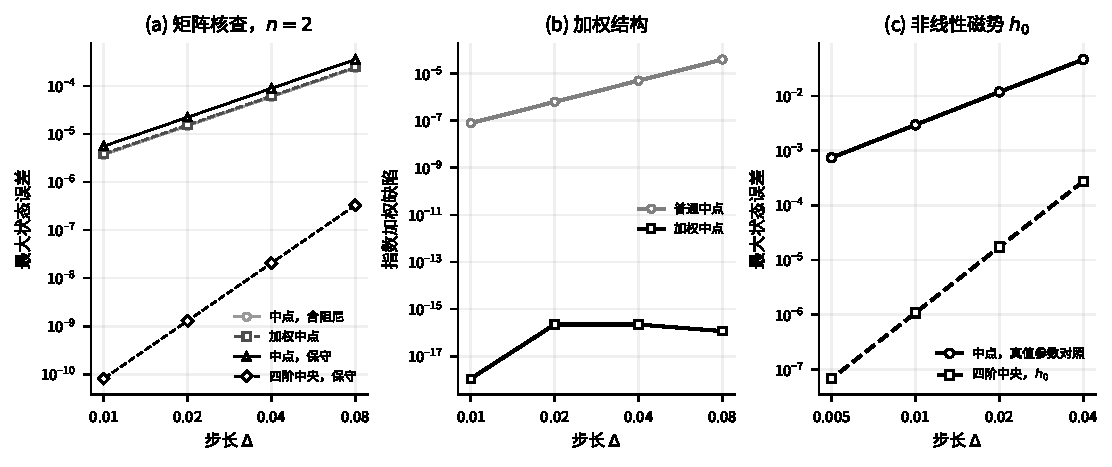
\includegraphics[width=\textwidth]{figures/framework_matrix_checks.pdf}
\caption{P1 的映射实现核查。(a) $n=2$ 时相对独立矩阵指数的全网格误差；含阻尼组与保守组分别采用各自声明的精确目标。(b) 普通与加权含阻尼中点法的指数加权缺陷。(c) 中点法与 Central4 作用于同一非线性保守磁模型 $h_0$；这些曲线比较的是同一个哈密顿量的不同离散方法。全部坐标、矩阵、初态及参考设置均记录在 JSON 中。}
\label{num:matrix-structure}
\end{figure*}

\subsection{共同物理基准与模态坐标}
\label{num:fe}
基准采用配套的材料参考值 $E\simeq2.1$ MPa 与 $\rho\simeq1028$ kg/m$^3$，并遵循 \citet{cho2021pdms} 所述的制备条件。自由长度 $80$ mm 和半径 $0.6$ mm 是研究设计输入。标称边长 $0.250$ mm 的立方磁芯采用 $B_r=1.425$ T 和密度 $7500$ kg/m$^3$，并保留其制造商牌号规格与标称选值的来源性质 \citep{smN50,kjMoment}。磁芯平动质量与转动惯量在降阶前计入有限元质量矩阵。将一致质量离散下 $16/32/64$ 个单元的频率与独立连续体边界方程根比较。前四阶模态的最大相对误差分别为 $9.59029\times10^{-6}$（$32$ 个单元）和 $6.02081\times10^{-7}$（$64$ 个单元）（表~\ref{sx:fe-table}）。

采用的 $32$ 单元坐标为
\begin{align}
 \omega_0=\omega_1&=7.84000916\ \mathrm{rad/s},\notag\\
 \omega_2&=47.39957662\ \mathrm{rad/s},\qquad
 \nu_2=6.04585730,\notag\\
 d&=\bigl(0.30722439,\,0.45042632\bigr)^{\mathsf T},\notag\\
 \ell&=\bigl(0.0189673443,\,0.0077534761\bigr)^{\mathsf T}\ \mathrm m.
 \label{num:scales}
\end{align}
生成函数、控制器和物理读出均采用相同映射。所声明基准 $C=\alpha M_{\mathrm{total}}$ 的参数为 $\zeta_1^{\mathrm d}=0.025$、$\alpha=0.3920004581$ s$^{-1}$ 和 $\gamma=0.05$，由此得到 $\zeta_2^{\mathrm d}=0.0041350629$。这些阻尼比是设计选择，并非所声明梁的实测损耗。材料、惯量及剩磁的敏感性点另见表~\ref{sx:sensitivity-table}；它们不是置信区间，也不构成高模态控制验证。

\subsection{P2：通过磁端口实现学习残差补偿}
\label{num:p2}
\label{num:route-a}
相对 $h_0$ 的受控合成偏差由一个势能特征给出。定义
\begin{equation}
 \begin{split}
 \phi(X)&=\nabla_X g(d^{\mathsf T}X)\\
        &=d[\sin(d^{\mathsf T}X)-d^{\mathsf T}X],
 \end{split}
 \label{num:feature-gradient}
\end{equation}
以及
\begin{equation}
 \begin{split}
 R_*(X)&=\beta_*g(d^{\mathsf T}X),\qquad \beta_*=0.2,\\
 \widehat R(X)&=\widehat\beta g(d^{\mathsf T}X).
 \end{split}
 \label{num:feature}
\end{equation}
系数 $0.2$ 是明确声明的压力测试设置，并非辨识得到的材料偏差。加上阻尼系数后，待拟合量只有两个标量。恢复这两个系数并不衡量完整 CHNN 优化，也不衡量对更丰富残差族的泛化。

\label{num:identification}
四条训练轨迹和两条独立验证轨迹各持续 $\tau=4$。每隔 $0.002$ 观测一次无噪声状态，采用长度为 $0.04$ 的 Simpson 积分窗，得到 $400$ 个训练向量增量，即 $800$ 个标量行。对于 $W=[\tau_a,\tau_b]$，积分平衡为
\begin{equation}
 \begin{split}
 b_W&=Y_b-Y_a+\int_W\{\mathsf NX+\phi(X)\}\,\mathrm d\tau,\\
 A_W&=\left[-\int_W\phi(X)\,\mathrm d\tau,
                 -\int_WY\,\mathrm d\tau\right],\\
 A_W\binom{\beta}{\gamma}&\simeq b_W.
 \end{split}
 \label{num:regression}
\end{equation}
经列缩放的无约束最小二乘给出
\begin{equation}
 \widehat\beta=0.200003368491,\qquad
 \widehat\gamma=0.04999999998680.
 \label{num:fitted-values}
\end{equation}
训练与留出验证的增量 RMS 残差分别为 $1.0123\times10^{-12}$ 和 $9.2492\times10^{-13}$。原始与缩放后设计矩阵的条件数分别为 $10418.25$ 和 $1.04537179$。归一化 Gram 矩阵满足 $\lambda_{\min}(G)=5.15486\times10^{-14}$，因此即使缩放后的求解条件良好，弱特征激励仍然重要。依赖真值计算的系数误差 $3.36849\times10^{-6}$ 是合成诊断量；第~\ref{sec:kam}~节的解析估计仍需要独立论证的积分与观测缺陷上界。

四个恢复组均从 $(0.09,0.08,0.015,-0.01)$ 出发，积分至 $\tau=20$（$2.551017$ s），中点步长为 $0.001$。每个非零指令都在积分过程中转换为物理磁力／磁力矩及场／梯度，经重构后代回受控对象。只有明确标出的真值参数对照使用真实系数。各组均与从相同初态独立积分得到的 $h_0$ 轨迹比较。

\begin{table*}[t]
\centering
\caption{P2 通过同一物理端口映射恢复目标。状态与末端 RMS 采用独立的 $h_0$ RK4 参考；能量变化为无量纲标称量 $\max_k|h_0(x_k)-h_0(x_0)|$。}
\label{num:a-table}
\begin{tabular}{lccc}
\toprule
控制 & 状态 RMS & 末端 RMS ($\mu$m) & 最大标称能量变化\\
\midrule
无控制 & $2.92453\times10^{-2}$ & $322.376137$ & $1.50142\times10^{-2}$ \\
阻尼补偿 & $2.43437\times10^{-5}$ & $0.143531$ & $1.37056\times10^{-7}$ \\
学习恢复 & $1.71438\times10^{-5}$ & $0.094120$ & $5.64520\times10^{-12}$ \\
真值参数恢复 & $1.71439\times10^{-5}$ & $0.094120$ & $3.24493\times10^{-12}$ \\
\bottomrule
\end{tabular}
\end{table*}

在该理想两模态实验中，拟合得到的恢复控制将状态 RMS 降至 $1.71438\times10^{-5}$，末端 RMS 降至 $0.094120\,\mu$m。其采样连续向量场失配 RMS 为 $2.5942\times10^{-11}$，但轨迹误差仍接近真值参数对照的 $1.71439\times10^{-5}$，因为二者包含相同的中点相位误差。学习组略小的误差可以由两种小误差相互抵消产生，不能作为优于真实参数控制的证据。这里检验的是从共同初态恢复目标轨迹，而非从跟踪偏移出发的吸引性。

\subsection{P3：向实际受控动力学的收敛}
\label{num:p3}
\label{num:integration}
保留主要的非线性真值参数中点对照。以 $0.04,0.02,0.01,0.005$ 逐次减半步长，最终观测阶为 $1.999331$，比较基准为独立 RK4 参考；该参考的步长加密差异为 $6.3600\times10^{-12}$。新增 Central4 实验采用同一个完整余弦保守 $h_0$，其全部导数见补充材料式~\eqref{ss:central4-magnetic-jacobian}；该方法并非在无关映射之后追加控制跳变。最终观测阶为 $3.999503$。独立 DOP853 参考加密差异为 $1.1642\times10^{-11}$，低于所报告的最小 Central4 误差。解析增量 Jacobian 在指定核查状态处与复步长微分的最大差异为 $2.7756\times10^{-17}$。

\begin{table*}[t]
\centering
\caption{非线性保守 $h_0$ 积分至 $\tau=20$。误差取全部保存时刻相对独立参考的最大值。中点法对应已有的完全补偿实验；Central4 对应新增保守格式核查。}
\label{num:nonlinear-order}
\begin{tabular}{rcccc}
\toprule
$\Delta$ & 中点误差 & 中点观测阶 & Central4 误差 & Central4 观测阶\\
\midrule
$0.04$ & $4.64310\times10^{-2}$ & --- & $2.75432\times10^{-4}$ & --- \\
$0.02$ & $1.18409\times10^{-2}$ & $1.971306$ & $1.73275\times10^{-5}$ & $3.990559$ \\
$0.01$ & $2.96760\times10^{-3}$ & $1.996414$ & $1.08474\times10^{-6}$ & $3.997648$ \\
$0.005$ & $7.42245\times10^{-4}$ & $1.999331$ & $6.78193\times10^{-8}$ & $3.999503$ \\
\bottomrule
\end{tabular}
\end{table*}

为区分数值收敛与模型恢复，另设实验固定非零辨识误差 $\delta\beta=0.02$、$\delta\gamma=0.01$。因此，同一声明受控对象上的控制器采用 $\widehat\beta=0.18$、$\widehat\gamma=0.04$。这些是人为设置的测试误差，并非前述拟合的输出或实测不确定性。实际向量场为
\begin{equation}
 \begin{split}
 X'&=\mathsf NY,\\
 Y'&=-\mathsf NX-(1+0.02)\phi(X)-0.01Y.
 \end{split}
 \label{num:fixed-error-field}
\end{equation}
中点闭环仍使用物理指令重构。独立的 DOP853 实现直接积分上述显式约化向量场；两种实现的采样向量场差异至多为 $1.1189\times10^{-16}$。所有步长均保持同一组控制系数不变。

\begin{table*}[t]
\centering
\caption{P3 的固定非零辨识误差实验。第一种误差相对同一实际连续闭环向量场计算；末列误差相对标称 $h_0$ 计算。二者均为全网格最大欧氏误差。}
\label{num:closed-convergence}
\begin{tabular}{rccc}
\toprule
$\Delta$ & 相对实际闭环的误差 & 观测阶 & 相对标称 $h_0$ 的误差\\
\midrule
$0.04$ & $4.20319\times10^{-2}$ & --- & $4.56736\times10^{-2}$ \\
$0.02$ & $1.07152\times10^{-2}$ & $1.971829$ & $1.60584\times10^{-2}$ \\
$0.01$ & $2.68521\times10^{-3}$ & $1.996545$ & $1.17602\times10^{-2}$ \\
$0.005$ & $6.71600\times10^{-4}$ & $1.999364$ & $1.14312\times10^{-2}$ \\
$0.0025$ & $1.67917\times10^{-4}$ & $1.999855$ & $1.14090\times10^{-2}$ \\
\bottomrule
\end{tabular}
\end{table*}

相对实际向量场的误差降至 $1.67917\times10^{-4}$，最终观测阶为 $1.999855$，而相对标称目标的误差趋于 $1.14090\times10^{-2}$。独立积分这两个连续模型，在最细公共网格上得到的最大差异为 $1.14070\times10^{-2}$。因此，减小步长能分辨实际闭环动力学，但不能消除所设置的建模误差。独立参考的加密差异为 $1.0636\times10^{-11}$。这一结果直接说明了收敛估计式~\eqref{ctrl:global-error} 的作用范围。

\label{num:defect-budget}
另用独立的单自由度谐振子诊断检验代数残差项。在二维相空间中，对中点增量方程人为加入 $r_k=0.01\Delta^q(1,0)^{\mathsf T}$、$q=1,2,3$，在 $T=4$ 上求解扰动后的方程。逐步保存原方程的每个实际残差。这是人为构造的代数缺陷，并非实测 Newton 停止误差，也不是导管实验。相对未扰动中点轨迹，新增误差的最终观测阶为 $0.000000,\,1.000000,\,2.000000$；它与 $\eta_\Delta/\Delta$ 的比值约为 $1.999999$。相对连续振子的总误差最终观测阶依次为 $0.000566,\,1.018776,\,1.999969$。其中 $q=3$ 保持二阶，而 $q=1$ 留下不消失的误差。该实验核查误差预算的缩放规律，并不确定定理常数的普适锐值。

\begin{figure*}[t]
\centering
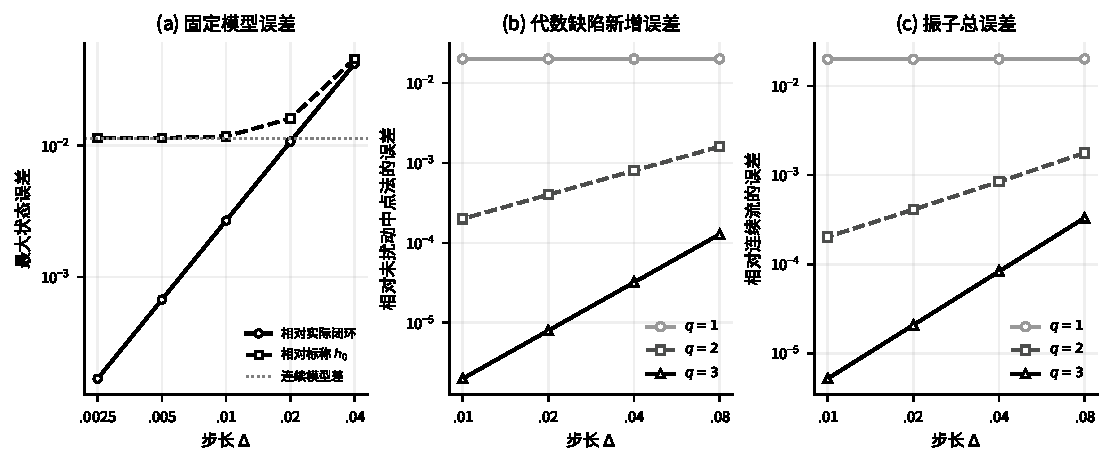
\includegraphics[width=\textwidth]{figures/framework_closed_loop_checks.pdf}
\caption{P3 区分数值误差与模型误差。(a) 固定 $\delta\beta=0.02$、$\delta\gamma=0.01$ 时，中点法收敛至实际闭环向量场，而其相对 $h_0$ 的误差趋于连续模型之差。(b) 人为增量缺陷引起的新增误差，以未扰动中点法为比较基准。(c) 相对独立连续振子的总误差；只有这项诊断采用独立的单自由度测试模型。}
\label{num:closed-results}
\end{figure*}

\subsection{阻尼情景、采样域与适用边界}
\label{num:damping}
对附加阻尼比 $\zeta_1^{\mathrm d}\in\{0,0.01,0.025,0.05,0.1\}$，分别重新生成训练／验证轨迹并重新拟合。恢复实验采用 $\tau\in[0,10]$、中点步长 $0.002$ 和独立 RK4 参考。表~\ref{sx:framework-damping-a} 给出无控制、学习及真值参数对照结果。这是模型族内的敏感性研究，并非检验一个冻结控制器抵抗未知阻尼变化。实际估计器明确采用无约束求解，并未隐式实现非负约束拟合。在真实阻尼为零时，它返回 $\widehat\gamma=-1.4038\times10^{-12}$；不将这一数值解释为材料具有负损耗。材料损耗依赖制备条件和频率，若无额外模型或器件测量，不能据此辨识这些模态阻尼比 \citep{fischer2017adhesion}。

\label{num:ports}
磁端口矩阵经列归一化后的条件数为 $3.8185963$；由于各列量纲不同，原始条件数不能被解释为与单位无关的指标。主要学习恢复实验的需求为 $\max|B_y|=0.544490$ mT 和 $\max\|\nabla B\|_2=0.01603429$ T/m。计入纵向偏置场后，最大局部磁场为 $30.004941$ mT。已发表磁系统可以提供场强量级的对照 \citep{lussi2021cvs}，但不能证明这些指令的联合场／梯度可实现性或带宽。采样末端角度与整梁斜率保持在所声明的小斜率诊断域内；这里没有认证连续时间或空间上的极值。

实验未执行饱和或输入功约束器。对于净 $4$ mm 间隙，$E_c=10.019717$ nJ，$0.95E_c=9.518731$ nJ，而主要实验的初始标称能量为 $12.656721$ nJ。因此，初始化时尚不满足所提出的充分能量上限前提。这些框架实验验证了矩阵一致性、特定收敛阶、代数磁端口实现及所述收敛区分。完整网络拟合、高模态受迫轨迹、COMSOL 对比、长时间频率研究和有限域 KAM 证书仍需单独完成。补充材料第~\ref{sx:migration}~节保留了这些早期结果的状态。

\section{补偿动力学的离散 KAM 持久性}\label{sec:kam}
\subsection{从非零积分损失到可控扰动}
\label{kam:learning-section}

长期行为问题针对补偿后导管的精确隐式映射。由命题~\ref{ctrl:structure-proposition}，当残余阻尼为零且广义输入以保守方式实现时，该映射精确辛。其哈密顿量为 $h_c=h_0+\delta R$，因此连接离散 KAM 需要在某个邻域上界定 $\delta R$，而不只是沿有限条轨迹吻合。\citet{chen2022} 的非零损失观点启发了这一连接。对于本文采用的有限特征读出，可以将其写成确定性的显式关系，无须假设训练残差为零，也不将实域预测误差当作解析范数。

令 $D,y$ 为式~\eqref{struct:integral-design} 中堆叠后的量，并记 $\theta_*=(\beta_*^{\mathsf T},\gamma)^{\mathsf T}$、$e=y-D\theta_*$。定义
\begin{equation}\label{kam:gram}
 G_I=\frac{D^{\mathsf T}D}{nL_I},\qquad
 r_I=\frac{\norm{D\widehat\theta-y}_2}{\sqrt{nL_I}}.
\end{equation}
缺陷 $e$ 包含观测重构、输入标定、数值求积和模型类误差。假设独立估计对实际使用的矩阵给出
$\norm e_2/\sqrt{nL_I}\le\epsilon_I$ 及
$\lambda_{\min}(G_I)\ge\underline\lambda>0$，则有
\begin{equation}\label{kam:integral-bound}
 \norm{\widehat\theta-\theta_*}_2
 \le b_I:=\frac{r_I+\epsilon_I}{\sqrt{\underline\lambda}}.
\end{equation}
事实上，$D(\widehat\theta-\theta_*)=(D\widehat\theta-y)+e$，而 $D/\sqrt{nL_I}$ 的最小奇异值给出其左端范数的下界。该论证适用于任意拟合系数，包括带约束的阻尼估计。增加观测量只有在改善缺陷界或改善 $G_I$ 所反映的激励程度时才有帮助。

令 $\mathcal U\subset\C^{2n}$ 为真实工作域 $K$ 的指定复邻域，定义
\begin{equation}\label{kam:feature-bounds}
\begin{aligned}
 B_F(\mathcal U)&=\left(\sum_j\norm{F_j}_{\mathcal U}^{2}\right)^{1/2},\\
 B_{\nabla F}(K)&=\left(\sum_j\sup_K\norm{\nabla F_j}_2^2\right)^{1/2}.
\end{aligned}
\end{equation}
若 $R_*=\sum_j\beta_{*,j}F_j+R_{\rm out}$，由 Cauchy--Schwarz 不等式得
\begin{equation}\label{kam:analytic-error}
\begin{aligned}
 \norm{\delta R}_{\mathcal U}
    &\le b_I B_F(\mathcal U)+\norm{R_{\rm out}}_{\mathcal U},\\
 \sup_K\norm{\nabla\delta R}_2
    &\le b_I B_{\nabla F}(K)+\sup_K\norm{\nabla R_{\rm out}}_2,\\
 |\delta\gamma|&\le b_I.
\end{aligned}
\end{equation}
第一行是 KAM 所需的能量扰动预算，第二、三行则进入跟踪方程。在较小复域上的导数界也可由 Cauchy 估计得到，并显式依赖于缩减的域宽。独立控制的 $R_{\rm out}$ 必须同时计入观测缺陷和这些函数界。对合成的单特征受控对象，该项为零。第~\ref{sec:analysis} 节报告的基于数值真值的缺陷，是对该实验的诊断；严格证书或实验验证还需要经过验证的不确定性界。

\subsection{实解析性与正确的复延拓}
\label{kam:analyticity}

采用复状态坐标本身并不意味着满足解析性假设。能量在 $(X,Y)\in\R^{2n}$ 上为实值，其延拓关于 $2n$ 个独立复变量 $(X,Y)$ 全纯，等价地，也关于独立的 $(\zeta,\chi)$ 全纯。在物理实切片上满足 $\chi=\bar\zeta$，但在延拓域中求导时不施加这一共轭关系。例如，
\begin{equation}\label{kam:complex-energy}
\begin{aligned}
 h_0^{\C}(\zeta,\chi)
  ={}&\sum_j\nu_j\zeta_j\chi_j
      +1-\cos\!\left(\frac{d^{\mathsf T}(\zeta+\chi)}{\sqrt2}\right)\\
     &-\frac{[d^{\mathsf T}(\zeta+\chi)]^2}{4}.
\end{aligned}
\end{equation}
这是物理实值能量的延拓，并非仅关于 $\zeta$ 的全纯函数。将
$\zeta'=-\mathrm i h_\chi^{\C}$ 与
$\chi'=\mathrm i h_\zeta^{\C}$ 限制到实切片，即得到对应的物理哈密顿方程。

对神经网络读出，每一步运算都必须在选定域上具有全纯延拓。多项式与余弦特征满足这一要求。亚纯激活函数要求所选域避开其极点；分段线性激活函数不满足这里使用的解析 KAM 版本。输出端的取实部操作，应通过独立变量中的共轭对称系数进行延拓，而不是在复域内施加非全纯的取实部操作。补充材料~\ref{ss:analytic-extension} 给出这一构造。真实残差与学习残差都必须具备所声明的正则性。有限次可微 KAM 定理是另一种选择，其可微性和范数假设不同；本基准不调用该类定理。

\subsection{真正的局部作用--角模型及其扭转矩阵}
\label{kam:normalform-section}

平衡变量已经将正定二次能量对角化为 $h_2=\tfrac12\sum_j\nu_j(X_j^2+Y_j^2)$。极坐标
$X_j=\sqrt{2I_j}\cos\phi_j$、
$Y_j=-\sqrt{2I_j}\sin\phi_j$
是正则坐标，并给出 $h_2=\nu\cdot I$。其中的径向变量 $I_j$ 并不是耦合余弦哈密顿量的精确作用变量。在分离可积部分与余项之前，需要构造近恒等的正则正规形变换。

为计算标称扭转矩阵，在标量族中取 $\kappa=1$，该族为 $h_\kappa=h_2+\kappa g(d^{\mathsf T}X)$。其四次项为 $h_{4,\kappa}=-\kappa(d^{\mathsf T}X)^4/24$。假设
$k\cdot\nu\ne0$ 对 $0<|k|_1\le4$ 成立，则四次同调方程
\begin{equation}\label{kam:homological}
 \{h_2,W_{4,\kappa}\}
    =-(h_{4,\kappa}-\langle h_{4,\kappa}\rangle)
\end{equation}
存在多项式解；泊松括号约定为
$\{f,g\}=\nabla f^{\mathsf T}J\nabla g$。
该解的局部 Hamiltonian 流，再接上正作用量域内的极坐标参数化，定义正则坐标图 $\mathcal T_\kappa$。直接作角平均得到
\begin{equation}\label{kam:magnetic-twist}
\begin{aligned}
 h_\kappa\circ\mathcal T_\kappa
       &=H_{\rm NF}^{\kappa}(I)+R_6^\kappa(I,\phi),\\
 H_{\rm NF}^{\kappa}(I)
       &=\nu\cdot I+\tfrac12I^{\mathsf T}A_\kappa I,\\
 A_\kappa&=-\frac{\kappa}{8}
 \begin{pmatrix}
 d_1^4&2d_1^2d_2^2\\
 2d_1^2d_2^2&d_2^4
 \end{pmatrix},\\
 \det A_\kappa&=-\frac{3\kappa^2d_1^4d_2^4}{64}.
\end{aligned}
\end{equation}
其中非对角项不可缺少。当 $\kappa d_1d_2\ne0$ 时，扭转矩阵不定且非奇异；Kolmogorov 非退化要求可逆，并不要求正定。对于新基准，直接浮点计算得到
$\det A_1\simeq-1.719\times10^{-5}$ 及
$\sigma_{\min}(A_1)\simeq2.065\times10^{-3}$。这些是可复现的代数检验，不是环面的区间界。四次阶以内的有限非共振检验，也不同于下文对所有整数向量要求的小除数条件。

由于能量及四次变换保持偶次结构，余项关于笛卡尔坐标振幅从六阶起始。它既包含原余弦函数的尾项，也包含变换产生的泊松括号项。特别地，$W_{4,\kappa}=\kappa W_{4,1}$ 会产生正比于 $\kappa^2$ 的项，因此不能仅将标称尾项估计乘以 $\kappa$ 来得到完整余项。补充材料~\ref{ss:normalform} 给出该构造，以及存在三次项时的扩展。

\subsection{受控正规形及其扰动预算}
\label{kam:closed-budget-section}

标称坐标图 $\mathcal T_1$ 由补偿控制器所要恢复的同一耦合余弦能量构造。将其用于实际保守闭环，得到
\begin{equation}\label{kam:closed-budget}
\begin{aligned}
 h_c\circ\mathcal T_1
    &=H_{\rm NF}^{1}(I)+P_c(I,\phi),\\
 P_c&=R_6^{1}+\delta R\circ\mathcal T_1,\\
 \epsilon_c&=\norm{R_6^{1}}_{\mathcal D_c}+b_R^c,\\
 \norm{\delta R\circ\mathcal T_1}_{\mathcal D_c}&\le b_R^c.
\end{aligned}
\end{equation}
选择正作用量域 $\mathcal I_c\Subset(0,\infty)^2$、其复作用量邻域和一个复角条带，合记为 $\mathcal D_c$。在所用定义域上，坐标图及其逆必须解析，且导数有界；它们的实像须位于力学工作域内。只有坐标图的像包含于同一个已有界控制的物理复邻域中，才能将式 \eqref{kam:analytic-error} 的函数界转化为 $b_R^c$。

式 \eqref{kam:closed-budget} 包含两类误差：标称正规形余项和保守辨识误差。即使精确辨识，仍有 $R_6^1$；仅有较小的数据损失，不能界定其中任一项。前述 $A_1$ 的奇异值计算构成代数非退化性检验；要在有限幅度上应用 KAM，还需要定义域余量、完整余项和逆坐标图的界。该矩阵无须正定，但小量检验不能省略其最小奇异值和逆矩阵范数。

学习得到的保守参考采用不同的比较能量：$\widehat h-h_*=-\delta R$；补偿闭环则满足 $h_c-h_0=\delta R$。补充材料~\ref{sec:supp-tracking} 保留了这一区分以及独立的参考跟踪分析。下述主要离散定理针对 $h_c$ 及标称正规形，不以 $\widehat h$ 替换其目标。

\subsection{实际受控数值映射的持续存在结论}
\label{kam:map-section}

设 $\Psi_\Delta^c$ 为精确求解式 \eqref{ctrl:midpoint} 所定义的映射，其中 $\delta\gamma=0$；也可取由完整 $h_c$ 生成的 Central4 映射。其解析性要求在适当复邻域上存在唯一隐式分支。配合保证端点及映射像留在该邻域内的余量，一个充分的局部条件为
\begin{equation}\label{kam:implicit-branch}
 \tfrac12\sup\norm{J S_\Delta''}<1.
\end{equation}
对于中点法，该条件为 $\Delta\sup\norm{J\nabla^2h_c}/2<1$。它与补充材料~\ref{ss:projection} 中端点投影和 Newton 矩阵所需的可逆条件相同。式 \eqref{ctrl:exact-primitive} 证明的精确性在解析正则正规形坐标图变换下仍保持，包括周期作用角环域上的情形。

需要分析的数值映射是
$\mathcal T_1^{-1}\circ\Psi_\Delta^c\circ\mathcal T_1$。
它通常不同于先作非线性坐标变换再应用中点法。令
$\mathcal R_\Delta(I,\phi)=(I,\phi+\Delta\omega_0(I))$，
其中 $\omega_0=\nabla_I H_{\rm NF}^{1}$。在共同且适当缩小的解析域上，局部一致性和流扰动估计给出
\begin{equation}\label{kam:map-closeness}
\begin{aligned}
 &\norm{\mathcal T_1^{-1}\Psi_\Delta^c\mathcal T_1
            -\mathcal R_\Delta}\\
 &\qquad\le C_1\Delta\epsilon_c+C_2\Delta^{p+1}.
\end{aligned}
\end{equation}
这里采用周期角变量的提升来比较映射，中点法对应 $p=2$，Central4 对应 $p=4$。这些常数需要相应定义域上的解析导数界和坐标图界。

精确辛性与可逆的混合端点投影共同给出单值周期生成扰动 $G_\Delta$，其基准为 $\Delta H_{\rm NF}^{1}$。缩小定义域后，估计为
\begin{equation}\label{kam:map-generator-budget}
 \norm{G_\Delta/\Delta}
       \le C_3\epsilon_c+C_4\Delta^p.
\end{equation}
按 $\Delta$ 归一化至关重要：每步生成函数误差为 $O(\Delta\epsilon_c+\Delta^{p+1})$，而映射定理中的小量为 $O(\epsilon_c+\Delta^p)$ \citep[Section~4]{shang}。减小步长仅能减少该预算中的离散化部分。

非共振条件同样是离散的。每步的角增量为 $\Delta\omega$，允许的频率须满足
\begin{equation}\label{kam:map-divisors}
 \left|e^{\mathrm i\Delta k\cdot\omega}-1\right|
       \ge\Delta\gamma_D|k|_1^{-\tau_D},
       \qquad k\in\mathbb Z^2\setminus\{0\}.
\end{equation}
这包含与 $2\pi$ 的整数倍发生的共振，因此，对指定步长和频率而言，连续非共振条件或有限整数扫描都不够。

\begin{proposition}[补偿后导管的条件性离散持续存在]
\label{kam:map-theorem}
假设命题~\ref{ctrl:structure-proposition} 中的保守实现条件成立，真实残差和学习残差实解析，式 \eqref{kam:closed-budget} 中的定义域与坐标图界成立，且精确隐式映射有唯一解析分支。设标称频率映射满足一致的扭转矩阵界
\[
 \iota\norm v_\infty\le\norm{D_I\omega_0(I)v}_\infty
                \le\Theta\norm v_\infty,
 \qquad0<\iota\le\Theta.
\]
选择 $0<\Delta\le1$、$\tau_D>3$，以及
$0<\gamma_D\le\min(1,\rho_I\Theta/2)$，
其中 $\rho_I$ 为复作用量半径。保留满足式 \eqref{kam:map-divisors} 且距频率域边界至少 $2\gamma_D$ 的频率。若相关常数及缩小后的解析域满足小量不等式
\begin{equation}\label{kam:map-smallness}
 C_3\epsilon_c+C_4\Delta^p
       \le\delta_0\gamma_D^2\iota^2\Theta^{-3},
\end{equation}
其中 $\delta_0$ 取自所用解析映射定理，则 $\Psi_\Delta^c$ 具有相应的拟周期不变环面 Cantor 族。正测度族的结论还需要该定理关于频率域几何与测度的假设。
\end{proposition}

\begin{proof}
四次正规形提供可积频率映射，式 \eqref{kam:closed-budget} 界定其 Hamiltonian 扰动。隐式分支与精确辛性在共轭后给出周期混合生成函数；一致性估计给出式 \eqref{kam:map-generator-budget}。该小量条件及所述离散小除数和频率余量，正是 \citet[Theorem~2 and Remark~2]{shang} 的解析假设，近可积应用见该文第~4 节。应用该定理，再通过 $\mathcal T_1$ 将不变环面共轭变换回原坐标，即得结论。补充材料~\ref{ss:map-kam} 列出混合生成方程和需要界定的常数。
\end{proof}

对于这一仿射频率映射，在所声明的定义域上可取
$\iota=\norm{A_1^{-1}}_\infty^{-1}$ 和
$\Theta=\norm{A_1}_\infty$。式 \eqref{kam:map-smallness} 给出的是待验证条件；当前基准尚未对依赖定理的常数、复余项和坐标图界进行数值认证。不能用测得的训练误差替代这些量。

\subsection{连续系统对照与结论范围}
\label{kam:scope}

连续哈密顿量 $h_c$ 有其独立的条件性 KAM 结论。它采用连续小除数 $|k\cdot\omega|\ge\gamma_D|k|_1^{-\tau_D}$，在两个自由度下允许取指数 $\tau_D>1$，并需要自身的解析小量条件 \citep{poschel}。命题~\ref{kam:flow-theorem} 位于补充材料~\ref{sec:supp-tracking}，给出了该对照及其对学习参考的扩展。它不替代离散小除数检验，也不将连续环面等同于某个指定数值映射的环面。当非零 $\epsilon_c$ 固定时，令 $\Delta\to0$ 既不会消除建模扰动，也不能证明数值环面收敛到近可积连续流的某个指定环面。

当前计算提供了更新后的物理与模态输入、冻结的系数辨识结果、有限数据诊断、四次扭转矩阵，以及理想隐式映射的代数结构。它们没有给出独立认证的观测缺陷界、完整复正规形余项或 KAM 阈值的数值核算。因此，命题~\ref{kam:map-theorem} 对当前基准仍是条件性结果。学习补偿计算保留非零阻尼误差，不能将该计算本身声明为精确辛映射；其有限时间数值收敛性则在命题~\ref{ctrl:convergence} 的假设下由该命题保证。

也可采用后验定理认证有限幅度环面，此时需要近似嵌入、其复条带上的不变性缺陷、Diophantine 频率，以及经过验证的扭转量和定义域界 \citep{haro2019aposteriori}。这些量需要针对当前参数重新计算，先前的环面证书不会自动转移。不变环面描述选定的有界离散运动，并不意味着任意初态都会被吸引到环面上。它们也不能保证整根柔性梁的净空；相应空间与驱动条件在第~\ref{sec:application} 节单独处理。

\section{磁输入实现与全梁验证}\label{sec:application}
应用目标是通过学习得到的残差补偿和阻尼补偿，恢复耦合的标称磁驱动运动。
物理输入映射必须实现式~\eqref{struct:route-a-control} 中的反馈，
保留其估计误差，并采用与式~\eqref{ctrl:midpoint} 相同的中点约定。
首先将这条链在两模态对象上闭合，再明确同一拟合控制器作用于更多梁模态时出现的附加项。
全梁净空论证则是关于物理能量的另一项条件。
对学习参考轨迹的跟踪保留为补充材料第~\ref{sec:supp-tracking} 节中的扩展。

\subsection{学习残差补偿的磁驱动实现}
\label{app:ports}
采用 $U=U_A=\widehat\gamma Y+\nabla\widehat R(X)$（见式~\eqref{struct:route-a-control}），求解
\begin{equation}
 \binom{F}{\tau_B}=A_{\rm mag}^{-1}\Lambda U.
 \label{app:port-inverse}
\end{equation}
连续输入 $U\in\mathbb R^2$ 无量纲；$F$ 和 $\tau_B$ 的单位分别为 N 和 N\,m。
式~\eqref{ctrl:midpoint} 中的四维离散增量还包含时间步长。
这些换算明确区分了物理力、连续广义输入和相空间增量。

这里 $\tau_B$ 是主动磁力矩。在两模态物理变量中，
第~\ref{sec:analysis} 节使用的合成受控对象为
\begin{align}
 \ddot a+\alpha\dot a+\Omega_2^2a
 &=\boldsymbol t E_0(\vartheta-\sin\vartheta)
       -\Lambda\nabla R_*(X)\nonumber\\
 &\quad+A_{\rm mag}\binom{F}{\tau_B},
 \qquad a=D_sX.
 \label{app:residual-plant}
\end{align}
由于 $\ddot a=\Lambda Y'$ 且
$\Lambda\nabla V_0=\Omega_2^2a+\boldsymbol tE_0(\sin\vartheta-\vartheta)$，
代入后恢复式~\eqref{struct:plant}。模态总力矩是另一种等价的端口约定：
\begin{align}
 T&=E_0(\vartheta-\sin\vartheta)+\tau_B,\nonumber\\
 A_{\rm mag}\binom{F}{T}
 &=\Lambda U+\boldsymbol tE_0(\vartheta-\sin\vartheta).
 \label{app:total-port}
\end{align}
偏置场余项是已知的，而真实残差力 $-\Lambda\nabla R_*$ 仍保留在受控对象中。
控制器不会通过这一约定变换读取 $R_*$。

将学习控制律代入物理受控对象，得到
\begin{align}
 \ddot a&=-\Lambda\nabla V_0
       +(\widehat\alpha-\alpha)\dot a\nonumber\\
       &\quad-\Lambda\nabla\delta R,\nonumber\\
 \widehat\alpha&=\omega_0\widehat\gamma,\qquad
 \delta R=R_*-\widehat R.
 \label{app:physical-closed-loop}
\end{align}
因此，物理闭环与式~\eqref{struct:route-a-closed} 保留了相同的势能误差和阻尼误差。
补偿目标保留完整耦合的标称磁势。
真值参数对照仅利用已知合成参数，区分数值误差与辨识误差。

令平面内的磁偶极矩为 $m=\mu(\cos\vartheta,\sin\vartheta,0)^{\mathsf T}$。
可提供所需力和磁力矩的局部磁场为
\begin{align}
 B(r)&=(B_0,B_y,0)^{\mathsf T}+G(r-r_{\rm tip}),\nonumber\\
 B_y&=\frac{\tau_B}{\mu\cos\vartheta},\nonumber\\
 G&=\frac{F}{\mu}
 \begin{pmatrix}
 -\sin\vartheta&\cos\vartheta&0\\
 \cos\vartheta&\sin\vartheta&0\\
 0&0&0
 \end{pmatrix}.
 \label{app:field-gradient}
\end{align}
直接相乘可得 $Gm=(0,F,0)^{\mathsf T}$ 和 $\|G\|_2=|F|/\mu$。
对称性与零迹分别满足局部无源区域的旋度和散度条件 \citep{abbott}。
主动磁力矩为 $\mu B_y\cos\vartheta$；轴向偏置磁力矩
$-\mu B_0\sin\vartheta$ 仍保留在储能模型中。

各补偿消融组均通过同一接口。
对于学习组，由磁场和梯度重构实际施加的横向力和主动磁力矩，并形成
\begin{align}
 U_{\rm rec}&=\Lambda^{-1}A_{\rm mag}
                    \binom{F_{\rm app}}{\tau_{B,\rm app}},\nonumber\\
 e_{\rm port}&=U_{\rm rec}-U_A(X,Y).
 \label{app:input-reconstruction}
\end{align}
理想精确换算给出 $e_{\rm port}=0$。
标定误差、角度估计误差、电流限制和饱和均可能使该量非零；
输入重构检验必须在实际施加到受控对象的输入中保留这些影响。
本文报告的测试验证局部代数换算，未实现饱和。

该接口要求 $A_{\rm mag}$ 的秩为二，角度定义域中的 $|\cos\vartheta|$
具有远离零的正下界，且联合磁场--梯度指令可行。
标称矩阵的列归一化给出条件数 $3.8186$，这是一项几何诊断。
物理驱动能力核算则需要按可用力和力矩缩放各列，并使用已辨识的线圈电流分配关系。
单一均匀磁场只提供一个模态输入方向。

偏置场和横向场按矢量模长合成：$30$ mT 偏置场叠加 $6$ mT 横向分量
需要 $30.594$ mT 的总场，而叠加 $20$ mT 横向分量则需要 $36.056$ mT。
已发表的 OctoMag 装置任意方向 $40$ mT 磁场能力 \citep{lussi2021cvs}
为这一场强尺度提供依据，但不能据此确定本文设计中可同时满足的梯度、工作空间或带宽限制。
学习残差补偿测试所需横向场峰值约为 $0.54449$ mT。
第~\ref{sec:analysis} 节报告了其输入重构与采样运行域检查。

\subsection{同一控制器作用于增加保留模态的受控对象}
\label{app:full-model}
固定 $32$ 单元梁的质量归一化特征基。
保留 $N\in\{2,4,8,64\}$ 个模态时，改变受控对象，而拟合后的两模态反馈保持不变。
记 $a^{(N)}=(a_1,\ldots,a_N)^{\mathsf T}$，
以 $\boldsymbol b_N,\boldsymbol t_N$ 汇集对应的端部系数。定义
\begin{align}
 \vartheta_N&=\boldsymbol t_N^{\mathsf T}a^{(N)},\nonumber\\
 A_{\rm mag}^{(N)}&=[\boldsymbol b_N\ \boldsymbol t_N]
                         \in\mathbb R^{N\times2},\nonumber\\
 X&=D_s^{-1}a_{1:2},\nonumber\\
 Y&=\omega_0^{-1}\mathsf N^{-1}D_s^{-1}\dot a_{1:2}.
 \label{app:enriched-coordinates}
\end{align}
这里 $D_s,\mathsf N$ 和 $A_{\rm mag}$ 仍表示固定的低模态映射。
$A_{\rm mag}^{(N)}$ 的前两行为 $A_{\rm mag}$；
两个物理端口无法独立指定全部 $N$ 个模态力。

此时必须将完整保守残差明确为物理势能 $\mathcal R_N(a^{(N)})$，以焦耳计。
模态扩展后的受控对象为
\begin{align}
 &\ddot a^{(N)}+\alpha\dot a^{(N)}+\Omega_N^2a^{(N)}\nonumber\\
 &\quad=\boldsymbol t_NE_0(\vartheta_N-\sin\vartheta_N)
       -\nabla_a\mathcal R_N\nonumber\\
 &\qquad+A_{\rm mag}^{(N)}\binom{F_{\rm app}}{\tau_{B,\rm app}}.
 \label{app:enriched-plant}
\end{align}
对于模型类匹配的合成层级，将同一个已声明的完整势能限制到各模态子空间，
使其满足 $\mathcal R_N(D_sX,0)=E_0R_*(X)$。
该条件并不意味着已经从两模态数据中辨识出完整势能。
补充材料~\ref{sm:enriched} 给出显式延拓与低模态投影。

令 $\vartheta_2=d^{\mathsf T}X$，定义两个附加项
\begin{align}
 e_{\rm mag}^{(N)}
 &=d[\vartheta_N-\sin\vartheta_N\nonumber\\
 &\qquad-\vartheta_2+\sin\vartheta_2],\nonumber\\
 e_R^{(N)}
 &=\Lambda^{-1}\nabla_{a_{1:2}}\mathcal R_N(a^{(N)})\nonumber\\
 &\quad-\nabla R_*(X).
 \label{app:enriched-defects}
\end{align}
在学习控制律保持不变时，精确低模态方程变为
\begin{align}
 X'&=\mathsf N Y,\nonumber\\
 Y'&=-\nabla(V_0+\delta R)(X)-\delta\gamma Y\nonumber\\
   &\quad+e_{\rm mag}^{(N)}-e_R^{(N)}+e_{\rm port}.
 \label{app:enriched-closed-loop}
\end{align}
磁场换算使用实际完整端角 $\vartheta=\vartheta_N$；
将其替换为两模态估计也可能产生 $e_{\rm port}$。
即使端口反演精确，高模态造成的端角差和残差差异也不会消失。
因此，仅有很小的两模态训练损失，既不能给出截断误差界，
也不能提供完整受控对象的 KAM 分析所需的哈密顿结构。

\subsection{分阶段完整模型验证方案}
\label{app:staged-validation}
后续验证阶段保持拟合系数、低模态初始状态、参考 $h_0$ 轨迹和端口约定不变。
在每一阶段，无控制、仅阻尼补偿、学习补偿和真值参数对照组均采用同一受控对象、
状态信息和执行器约束。
真值参数对照保留其两模态补偿律，与下述更强的全状态反馈有别。
即使高模态初始坐标为零，也仍可能产生响应，因为同一对端口作用于每个保留模态。
表~\ref{app:validation-stages} 区分了已完成的数值核查与拟开展的模态扩展。
$16/32/64$ 个单元的网格收敛检验针对线性空间离散；
改变保留模态数则检验受迫响应下的降阶模型与控制器。

\begin{table*}[t]
\centering\small
\caption{同一拟合残差控制器的分阶段验证。
高模态和独立有限元阶段属于明确的验证方案，并非本次新报告的仿真结果。}
\label{app:validation-stages}
\begin{tabular}{p{.15\textwidth}p{.45\textwidth}p{.30\textwidth}}
\toprule
阶段 & 固定对象与受控变化 & 状态及所需输出\\
\midrule
两模态 & 固定动能的残差类、一次联合拟合、共同的中点格式和磁接口 & 已完成：相对于独立参考解的误差、步长收敛、输入重构和采样指令需求。\\
$4$ 和 $8$ 个模态 & 同一 $32$ 单元基，固定学习控制律；将已声明的完整残差作一致限制；先取零高模态初始条件，再取指定的非零条件 & 计划开展：低模态状态误差、高模态响应及式~\eqref{app:enriched-closed-loop} 中的三类差项。\\
全部 $64$ 个模态 & 同一有限元质量、偏置刚度、端部磁芯惯量和物理端口；换算采用完整端角 & 计划开展：全中心线位移和斜率、输入峰值、初始化和启动瞬态。\\
独立有限元模型 & 在 COMSOL 或独立指定的求解器中重建相同几何、材料假设、端质量/转动惯量及边界载荷 & 计划开展：先验证线性模态，再在相同输入定义下比较受迫响应和降阶误差。\\
\bottomrule
\end{tabular}
\end{table*}

每次模态扩展运行应记录完整重构中心线、最大采样斜率、最小 $|\cos\vartheta_N|$、
状态 RMS 误差、端部误差、主频与组合频率、力/磁场/梯度峰值和饱和比例。
比较时间步长，并检查每个 Hermite 单元内的空间极值；
仅绘制端部轨迹不能界定梁其余部分的运动。
传感噪声、阻尼失配和限幅在另行声明的测试中引入，各控制器采用相同约束。
限幅后的指令必须实际施加到受控对象，并计入 $e_{\rm port}$，不能仍使用未限幅的广义力。

补充材料~\ref{sm:exact-lift} 保留了一项条件性不变环面构造，
其中更强的精确反馈使用已知阻尼和目标加速度。
当其全状态假设能够验证时，该定理具有作用，
但不能替代式~\eqref{app:enriched-closed-loop} 中保持不变的学习控制器。
本文不声称已经获得新的 $4/8/64$ 模态受迫轨迹、COMSOL 对比或有限幅度环面证书。

\subsection{由物理能量推得全梁净空}
\label{app:clearance}
令 $E(t)=H_0(q,M_f\dot q)$ 为式~\eqref{mech:fe-plant} 的物理能量。
对于任意满足固支条件的位移，
\begin{equation}
 w(s)=\int_0^s(s-\xi)w_{ss}(\xi)\dd\xi.
 \label{app:clamped-identity}
\end{equation}
由 Cauchy--Schwarz 不等式及动能、偏置场能量的非负性，得到
\begin{equation}
 \|w\|_\infty^2\le\frac{2L^3E_{\rm bend}}{3EI}
                    \le\frac{2L^3E}{3EI},\qquad
 E_c=\frac{3EIc^2}{2L^3}.
 \label{app:energy-bound}
\end{equation}
因此，$E<E_c$ 可保证整个中心线及其杆半径管状包络在所声明的直通道内满足净空要求。
该结果适用于任意容许位移形状，包括所有保留模态，并不限于静态端载荷形状。
对于本基准，$E_c=10.0197171$ nJ，所选能量上限为
$E_{\max}=0.95E_c=9.5187312$ nJ。

输入功约束器能够强制满足这一充分条件，而不必假设所要求的轨迹始终位于环面上。
令 $u=(F,B_y)^{\mathsf T}$，定义物理功率系数
\begin{equation}
 a_P=\binom{\dot w(L)}{\mu\cos\vartheta\,\dot\vartheta},\qquad
 W(0)\ge E(0),\quad \dot W=a_P^{\mathsf T}u.
 \label{app:work-observer}
\end{equation}
由式~\eqref{mech:physical-power}，有 $E(t)\le W(t)$。
给定期望指令 $u_{\rm req}$，在经尺度调整的正定度量 $R_u$ 下，选择最近的容许输入：
\begin{align}
 u=\mathop{\arg\min}_{\widetilde u\in\mathcal U(q)}
       &\ \tfrac12(\widetilde u-u_{\rm req})^{\mathsf T}
                 R_u(\widetilde u-u_{\rm req}),\nonumber\\
 \text{subject to }&\quad
 a_P^{\mathsf T}\widetilde u\le\kappa(E_{\max}-W),
 \qquad \kappa>0.
 \label{app:work-governor}
\end{align}
这里 $\mathcal U(q)$ 是包含零主动输入的非空闭凸联合端口可行集；
$R_u$ 考虑了力和磁场的不同单位。
若 $W(0)<E_{\max}$，则零输入可行，且
$E_{\max}-W(t)\ge[E_{\max}-W(0)]e^{-\kappa t}>0$。
结合式~\eqref{app:energy-bound}，即可证明满足该功率恒等式的解具有所需净空。
补充材料~\ref{sm:work} 将此论证扩展到给定的传感和执行误差界。
对于包含残差 $\mathcal R_N$ 的模态扩展受控对象，标称能量的导数还含有
$-\dot a^{(N)\mathsf T}\nabla_a\mathcal R_N$。
必须界定这一功率并将其纳入收支，或另行证明增广能量相对于弯曲能的下界。
标称净空定理不会自动包含该残差。
启用约束器可能改变所要求的哈密顿运动，因此净空证明与环面保持是不同的结论。

本文报告的残差补偿测试未使用该约束器。
其标称参考初始状态的能量为 $12.6567$ nJ，已经高于 $9.5187$ nJ 的上限。
因此，第~\ref{sec:analysis} 节中观测到的位移和斜率最大值属于数值运行域诊断，
并非上述能量上限保证的推论。
该约束器为未来从容许能量集合内部初始化的全状态实验提供了精确条件。

\section{结论}\label{sec:conclusion}
三个子问题已通过同一个耦合磁模型连接起来。对于 P1，比例阻尼的 Birkhoff 表示、相容端点投影和生成函数导出维度一致的加权映射。普通中点仍是作用于完整向量场的另一种实现。非交换矩阵消元保留质量、刚度和阻尼因子的运算次序；有效模态质量由明确的归一化推导得到，不能与组装后的梁质量矩阵混用。

对于 P2，积分观测在同一坐标系内辨识保守残差和阻尼。补偿保留标称余弦耦合，且每一组控制消融均经过相同的物理力--力矩及磁场--梯度接口。实际实现的闭环方程同时保留势能误差与阻尼误差。受限的无噪声实验检验了这一完整联系；较小的拟合残差并不构成一般 CHNN 训练性能或已标定物理器件的结论。

对于 P3，在隐式中点方程内加入反馈后，在局部光滑性、稳定性和定义域假设下，可得到对同一实际闭环的收敛。误差界包含累积增量残差，因此代数求解器容差和积分步长不能互相替代为精度指标。固定辨识误差则产生相对于标称目标的另一项偏差。精确辛性要求消除非保守残差；针对比例残余阻尼的加权格式保持相应的共形结构。离散 KAM 结论进一步要求解析性、扭转、非共振和小量假设；有限时间收敛与几何诊断本身不能自动建立这些假设。

修订后的材料与磁体记录为上述结论提供一致的物理基础。端部惯量、模态尺度、输入换算和能量净空界贯穿全文。扩展至更多保留模态时，必须保持已训练控制器，同时处理完整端角和明确给出的完整模型残差。在更强反馈假设下的精确全模态实现是另一项理论构造。当前两模态轨迹不能替代逐级验证，也不能替代实际执行的能量约束器。

尚需完成的实证工作包括试样辨识、联合磁场--梯度及感知标定，以及独立全阶模型或 COMSOL 检验。有限振幅 KAM 证书则要求在声明的定义域上验证解析余项和定理特定常数。因此，本文给出方向一的格式、控制器、受控收敛分析及可复现验证序列，同时明确保留这些后续认证要求。

\section*{数据与代码可用性}
随附源码包包含英文主稿、对应中文译稿、两份补充材料、参数记录，以及修订后的有限元、矩阵格式和受控离散计算脚本。在源码包根目录运行 \texttt{python3 reproduction/run\_all.py}，将先重新生成力学基准，再执行残差控制检验、相关跟踪扩展、阻尼扫描和研究框架验证组。上述计算需要 Python~3、NumPy 和 SciPy；重绘论文图表使用 Matplotlib。构建说明另列 PDF 编译步骤。

原稿来源为\href{https://github.com/mop74720-commits/IJRR_CHNN_KAM_v10_20261007}{公开 v10 仓库}，采用提交版本 \href{https://github.com/mop74720-commits/IJRR_CHNN_KAM_v10_20261007/tree/82519542dd057e8fbd6d6879ef33217761e8cbbb}{\texttt{82519542dd05}}，完整标识保存在随附来源记录中。该仓库的 S1/S2 档案继续作为原参数组的计算记录，不作为本次新生成的证据；本次修订也不声称复现全部历史结果。所提供的方向一研究框架决定本稿三个子问题的组织方式。源码包中的来源--章节对照表记录其格式、控制器、收敛论证和数值协议如何进入六节正文。此前的迁移表则单独说明哪些 v10 结果保留为一般理论、哪些已重新计算、哪些改为条件性陈述，以及哪些仅属于历史基准。

\section*{声明}
本文报告数学分析和计算机生成的力学数据。修订后的基准未开展人体、动物、硬件或在轨实验。材料参考值和制造商规格按各自性质引用，不据此暗示器件已经标定。本文件为沿用原论文章节与版式的研究修订稿，不构成发表或录用声明。

\begin{thebibliography}{99}

\bibitem[Abbott et~al.(2020)]{abbott}
Abbott JJ, Diller E and Petruska AJ (2020) Magnetic methods in robotics.
\textit{Annual Review of Control, Robotics, and Autonomous Systems} 3: 57--90.
\doi{10.1146/annurev-control-081219-082713}

\bibitem[Antman(2005)]{antman}
Antman SS (2005) \textit{Nonlinear Problems of Elasticity}. 2nd ed. Springer.
\doi{10.1007/0-387-27649-1}

\bibitem[Chen et~al.(2022)]{chen2022}
Chen Y, Matsubara T and Yaguchi T (2022) KAM theory meets statistical learning theory:
Hamiltonian neural networks with non-zero training loss.
\textit{Proceedings of the AAAI Conference on Artificial Intelligence} 36(6): 6322--6332.
\doi{10.1609/aaai.v36i6.20582}

\bibitem[Cho et~al.(2021)]{cho2021pdms}
Cho HS, Moon HY, Lee HS, Kim YT and Jeoung SC (2021) Formulation prediction for Young's modulus of poly(dimethylsiloxane) by spectroscopic methods.
\textit{Bulletin of the Korean Chemical Society} 42(9): 1225--1231. \doi{10.1002/bkcs.12352}

\bibitem[Desai et~al.(2021)]{desai}
Desai SA, Mattheakis M, Sondak D, Protopapas P and Roberts SJ (2021)
Port-Hamiltonian neural networks for learning explicit time-dependent dynamical systems.
\textit{Physical Review E} 104: 034312. \doi{10.1103/PhysRevE.104.034312}

\bibitem[Feng and Qin(2010)]{fengqin}
Feng K and Qin M (2010) \textit{Symplectic Geometric Algorithms for Hamiltonian Systems}. Springer.
\doi{10.1007/978-3-642-01777-3}

\bibitem[Feng et~al.(1989)]{feng}
Feng K, Wu HM, Qin MZ and Wang DL (1989) Construction of canonical difference
schemes for Hamiltonian formalism via generating functions.
\textit{Journal of Computational Mathematics} 7(1): 71--96.
\url{https://computmath.cjoe.ac.cn/jcm/EN/Y1989/V7/I1/71}.

\bibitem[Fischer et~al.(2017)]{fischer2017adhesion}
Fischer SCL, Kruttwig K, Bandmann V, Hensel R and Arzt E (2017) Adhesion and cellular compatibility of silicone-based skin adhesives.
\textit{Macromolecular Materials and Engineering} 302(5): 1600526. \doi{10.1002/mame.201600526}

\bibitem[Francescon et~al.(2025)]{francescon2025shape}
Francescon V, Murasovs N, Lloyd P, Onaizah O, Chathuranga DS and Valdastri P (2025)
Closed-loop shape-forming control of a magnetic soft continuum robot.
\textit{IEEE Robotics and Automation Letters} 10(6): 6071--6078.
\doi{10.1109/LRA.2025.3565124}

\bibitem[Greydanus et~al.(2019)]{greydanus}
Greydanus S, Dzamba M and Yosinski J (2019) Hamiltonian neural networks.
In: \textit{Advances in Neural Information Processing Systems}, vol. 32.
\url{https://arxiv.org/abs/1906.01563}.

\bibitem[Hairer et~al.(2006)]{hairer}
Hairer E, Lubich C and Wanner G (2006) \textit{Geometric Numerical Integration:
Structure-Preserving Algorithms for Ordinary Differential Equations}. 2nd ed. Springer.
\doi{10.1007/3-540-30666-8}

\bibitem[Haro and Luque(2019)]{haro2019aposteriori}
Haro \`A and Luque A (2019) A-posteriori KAM theory with optimal estimates for
partially integrable systems. \textit{Journal of Differential Equations}
266(2--3): 1605--1674. \doi{10.1016/j.jde.2018.08.003}
Preprint version used: \url{https://arxiv.org/abs/1711.05515v1}.

\bibitem[Hornik(1991)]{hornik}
Hornik K (1991) Approximation capabilities of multilayer feedforward networks.
\textit{Neural Networks} 4(2): 251--257. \doi{10.1016/0893-6080(91)90009-T}

\bibitem[Kim et~al.(2019)]{kim}
Kim Y, Parada GA, Liu S and Zhao X (2019) Ferromagnetic soft continuum robots.
\textit{Science Robotics} 4(33): eaax7329. \doi{10.1126/scirobotics.aax7329}

\bibitem[K\&J Magnetics(2026)]{kjMoment}
K\&J Magnetics (accessed 28 October 2026) Magnetic dipole moment.
\url{https://www.kjmagnetics.com/blog/magnetic-dipole-moment}.
Engineering dipole-moment approximation.

\bibitem[Lussi et~al.(2021)]{lussi2021cvs}
Lussi J et~al. (2021) A submillimeter continuous variable stiffness catheter for compliance control.
\textit{Advanced Science} 8(18): 2101290. \doi{10.1002/advs.202101290}

\bibitem[P\"oschel(2001)]{poschel}
P\"oschel J (2001) A lecture on the classical KAM theorem.
In: \textit{Proceedings of Symposia in Pure Mathematics}, vol. 69, pp. 707--732.
\doi{10.1090/pspum/069/1858551}
Preprint version used: \url{https://arxiv.org/abs/0908.2234v1} (Version 1.3, 2009).

\bibitem[Shang(1999)]{shang}
Shang ZJ (1999) KAM theorem of symplectic algorithms for Hamiltonian systems.
\textit{Numerische Mathematik} 83: 477--496. \doi{10.1007/s002110050460}

\bibitem[Simo(1985)]{simo}
Simo JC (1985) A finite strain beam formulation. The three-dimensional dynamic problem.
Part I. \textit{Computer Methods in Applied Mechanics and Engineering} 49(1): 55--70.
\doi{10.1016/0045-7825(85)90050-7}

\bibitem[SM Magnetics(2026)]{smN50}
SM Magnetics / SuperMagnetMan (accessed 28 October 2026) Magnet material grades: NdFeB stock grades, N50.
\url{https://supermagnetman.com/pages/magnet-material-grades}.
Manufacturer grade range, not an individual magnet calibration.

\bibitem[Su et~al.(2007)]{su2007}
Su HL, Sun YJ, Qin MZ and Scherer R (2007) Structure preserving schemes for Birkhoffian systems.
\textit{International Journal of Pure and Applied Mathematics} 40(3): 341--366.
\url{https://www.ijpam.eu/contents/2007-40-3/4/4.pdf}.

\bibitem[Tong et~al.(2025)]{tong2025navigation}
Tong D, Hao Z, Li J, Sun B, Liu M, Wang L and Huang W (2025)
Real-time simulation enabled navigation control of magnetic soft continuum robots in confined lumens.
\textit{Journal of the Mechanics and Physics of Solids} 203: 106198.
\doi{10.1016/j.jmps.2025.106198}

\bibitem[Trabelsi et~al.(2018)]{trabelsi}
Trabelsi C, Bilaniuk O, Zhang Y et~al. (2018) Deep complex networks.
In: \textit{International Conference on Learning Representations}.
\url{https://arxiv.org/abs/1705.09792}.

\bibitem[Zhang et~al.(2022)]{zhang}
Zhang SQ, Gao W and Zhou ZH (2022) Towards understanding theoretical advantages of
complex-reaction networks. \textit{Neural Networks} 151: 80--93.
\doi{10.1016/j.neunet.2022.03.024}
\href{https://www.lamda.nju.edu.cn/zhangsq/papers/2022-CRNet-NN.pdf}{Published version used for theorem numbering}.

\bibitem[Zhong et~al.(2020)]{zhong}
Zhong YD, Dey B and Chakraborty A (2020) Dissipative SymODEN: Encoding Hamiltonian
dynamics with dissipation and control into deep learning.
In: \textit{ICLR Workshop on Integration of Deep Neural Models and Differential Equations}.
\url{https://arxiv.org/abs/2002.08860}.
\end{thebibliography}

\end{document}
